% !TeX root = ../libro.tex
% !TeX encoding = utf8
% \lstdefinelanguage{JavaScript}{
%   keywords={typeof, new, true, false, catch, function, return, null, catch, switch, var, let, const, if, in, while, do, else, case, break},
%   keywordstyle=\color{blue}\bfseries,
%   ndkeywords={class, export, boolean, throw, implements, import, this},
%   ndkeywordstyle=\color{darkgray}\bfseries,
%   identifierstyle=\color{black},
%   sensitive=false,
%   comment=[l]{//},
%   morecomment=[s]{/*}{*/},
%   commentstyle=\color{green}\ttfamily,
%   stringstyle=\color{red}\ttfamily,
%   morestring=[b]',
%   morestring=[b]"
% }
\chapter{Desarrollo e implementación}
En esta sección veremos cómo se han usado las técnicas y conceptos presentados en los capítulos anteriores para la realización de una aplicación web que permita al usuario crear e interactuar superficies a través de SDFs, ecuaciones implícitas y paramétricas. El motivo de desarrollar una aplicación web es que sea accesible al mayor número de usuarios de la forma más cómoda posible. Se ha decidido usar React \cite{react} para esta tarea, una biblioteca de JavaScript (y TypeScript) para interfaces de usuario. Es una librería muy popular, y por tanto muy bien documentada y con muchos paquetes de la comunidad disponibles. Las principales características de React son:
\begin{itemize}
    \item Utiliza la \textbf{extensión de sintaxis} JSX, la cual permite escribir código JavaScript como si se tratase de HTML o XML. Se pueden usar expresiones JSX dentro de bucles \texttt{for} o entornos condicionales \texttt{if}, y dentro de ellas se pueden agregar expresiones JS entre corchetes. 
    \item Se basa en \textbf{componentes autocontenidos y reutilizables}. La forma más común actualmente de declarar componentes es a través de los llamados componente funcionales, los cuales reciben argumentos, o \texttt{props}, y devuelven una expresión JSX. Todos los componentes reciben el parámetro \texttt{children} por defecto, conteniendo la expresión JSX de los componentes que se encuentren entre las etiquetas de apertura y cierre del componente. El flujo de datos es unidireccional del componente padre a sus hijos.
    \item Utiliza un \textbf{DOM virtual} para solo actualizar los componentes cuyo estado o \texttt{props} han cambiado. En componentes funcionales, la manera de indicar variables que desencadenen un re-renderizado al ser modificadas es a través de \textit{hooks}. En general, estos son funciones de JS que permiten crear y acceder al estado y ciclos de vida de React. Los principales son \texttt{useState}, usado para declarar una variable junto con su \textit{setter}, y \texttt{useEffect}, que permite ejecutar código cuando se actualice el componente. Si solo se desea reaccionar a cambios de ciertos \textit{hooks}, este \textit{hook} permite indicar sus dependencias entre corchetes.
\end{itemize}
Un ejemplo de uso básico de JSX, componentes funcionales y manejo de estado en React sería el siguiente.
\begin{lstlisting}
function Tarjeta(props) {
  return (
    <div>
        {props.children}
        {props.nombre}
    </div>
  );
}

function Main() {
    const [miNombre, setMiNombre] = React.useState("Daniel");

    useEffect(()=>{
        console.log("Solo me ejecuto una vez al inicio");
    }, []);
    
    useEffect(()=>{
        console.log("Has cambiado el nombre");
    }, [miNombre]);
    
  return (
    <TarjetaNombre nombre={miNombre}>
      <h1>Hola, mi nombre es</h1>
    </TarjetaNombre>
  );
}
\end{lstlisting}
% Un aspecto fundamental a lo largo de todo el desarrollo será el del rendimiento ya que las aplicaciones web solo tienen a su disposición una hebra de ejecución (la de interfaz de usuario), haciendo de cuello de botella para el resto de cálculos.\newline

La aplicación consta de varios componentes principales que interaccionan entre sí, incluyendo un editor de nodos que permitirá aplicar operaciones sobre primitivas, un panel de creación y edición de primitivas, un lienzo sobre el que aplicar \textit{raymarching} y un gestor de estado. A continuación los estudiamos en detalle.

\section{Gestor de estado}
Empezamos hablando sobre el gestor de estado, ya que casi todos los demás componentes hacen uso y se comunican entre sí a través de él. Para esta tarea se ha hecho uso de Zustand \cite{zustand}, una librería de gestión de estado para JavaScript y TypeScript. Su funcionamiento consiste en el uso de contenedores, formados por atributos y métodos para trabajar con ellos. Cuando un componente quiere acceder a un contenedor, basta con que se suscriba a sus cambios a través del \textit{hook} que proporciona Zustand: \texttt{useStore}. Nosotros haremos uso de dos contenedores, uno para las primitivas definidas por el usuario y otro para gestionar el estado del editor de nodos. De este último hablaremos en la siguiente sección, pues solo es usado por el componente del editor de nodos. Sin embargo, el contenedor de primitivas es usado tanto por el editor de nodos como por el panel de primitivas, ya que ambos necesitan leer de él para saber cuales son las primitivas existentes, así como escribir para crear nuevas o modificar las existentes. Este contenedor tiene la estructura mostrada en la \autoref{fig:contenedorPrim}. En particular, la información se almacena a través del tipo \texttt{Primitive}, el cual tiene los siguientes atributos.
\begin{itemize}
    \item \texttt{name}: nombre que otorga a la primitiva el usuario y será mostrada por pantalla.
    \item \texttt{id}: identificador único obtenido aplicando normalización NFD a \texttt{name}.
    \item \texttt{inputMode}: indica el método que usó el usuario para definir la primitiva, ya sea introducir directamente la SDF con sintaxis GLSL, la ecuación implícita o la parametrización racional.
    \item \texttt{input}: cadena de texto con la ecuación introducida por el usuario. Dado que al usar parametrizaciones se requiere de tres ecuaciones, su valor se guarda en un array.
    \item \texttt{sdf}: función distancia con signo obtenida tras procesar la entrada del usuario.
    \item \texttt{parameters}: parámetros asociados a la primitiva y presentes en la función distancia con signo, que podrán ser usados en el editor de nodos para interactuar con ella. Cada parámetro viene representado por la estructura \texttt{Parameter}, que contiene el símbolo del parámetro presente en la expresión, una etiqueta para ser mostrado en el editor de nodos, y si su valor debe estar acotado en cierto rango. 
    \item \texttt{fHeader}: cabecera de la función GLSL asociada a la primitiva. La función tendrá como nombre el \texttt{id}, y recibe como argumentos el punto donde se quiera evaluar la SDF y cada uno de los parámetros en \texttt{parameters}.
    \item \texttt{material}: contiene las componentes especular, difusa y ambiental, así como el coeficiente de brillo del material asociado a la primitiva.
\end{itemize}
\begin{ejemplo}
Para definir una esfera centrada en el origen mediante su ecuación implícita y poder controlar su radio en el editor de nodos, se crearía la siguiente primitiva.
\begin{lstlisting}
{
  id: "sphere",
  name: "Sphere",
  inputMode: InputMode.Implicit,
  input: ["x^2 + y^2 + z^2 - r", "", ""],
  parsedInput: "length(p)-r",
  parameters: [
     { symbol: "r", label: "Radius", defaultVal: 1.0, type: "range", range:[0,100] }
  ],
  fHeader: "sphere(vec3 p, float r)",
  material: {
    specular: [1.0, 1.0, 1.0],
    diffuse: [0.0, 1.0, 0.0],
    ambient: [0.2, 0.2, 0.2],
    smoothness: 10.0
  }
}
\end{lstlisting}
\end{ejemplo}

\begin{figure}[ht!]
    \centering
    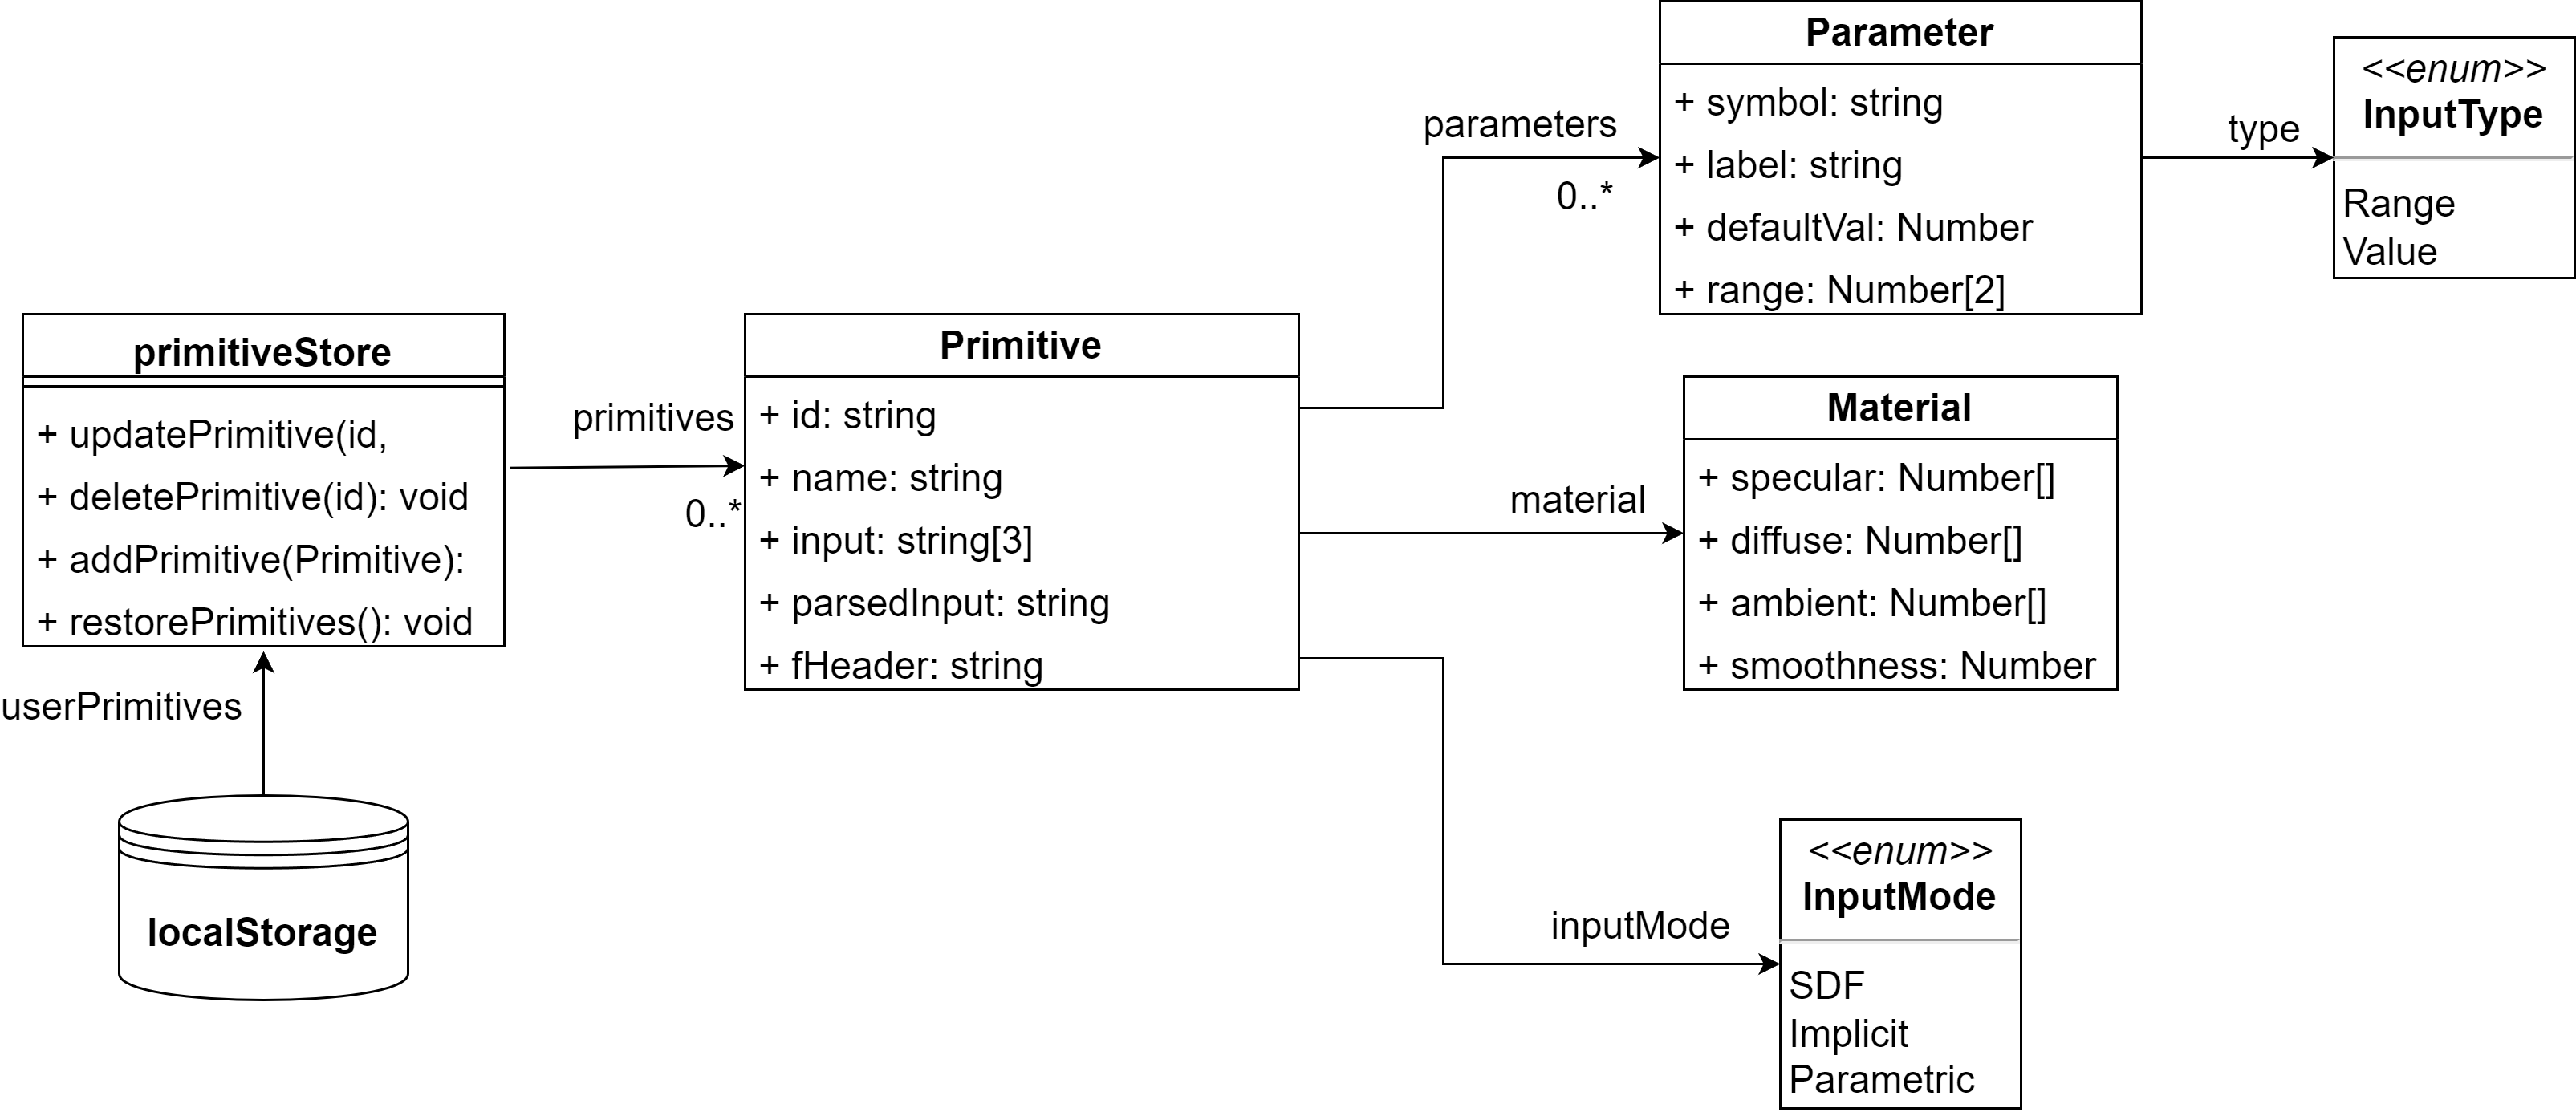
\includegraphics[width=\textwidth]{Plantilla-TFG-master/img/diagramaZustand.png}
    \caption{Diagrama de clases del contenedor de primitivas}
    \label{fig:contenedorPrim}
\end{figure}

Las principales ventajas de la elección de Zustand es que se trata de una librería de tamaño muy contenido, y al estar basada en \textit{hooks} solo actualizará los componentes que dependan de los cambios relevantes en el estado, haciendo la aplicación más eficiente. Además, siguiendo la filosofía de React, cada contenedor es autocontenido, siendo la única forma de acceder a los datos a través de los métodos del contenedor. Esto hace que sea más fácil debugear, así como evitar que haya modificaciones inesperadas desde algún componente externo. Por último, es muy sencillo almacenar la información del contenedor en el almacenamiento local a través del método \texttt{persist} incluido, de forma que el usuario pueda disponer de los datos guardados en sesiones anteriores.

\section{Lienzo}
Para poder mostrar al usuario el resultado de sus acciones a la hora de definir o aplicar operaciones sobre primitivas tenemos que poder visualizar una función distancia con signo mediante \textit{spheretracing}, aplicando los algoritmos de iluminación y renderizado vistos en el \autoref{cap:2}. Como se explicó en este capítulo, necesitaremos un lienzo con un \textit{vertex shader} y un \textit{fragment shader}. Tanto el lienzo como el \textit{vertex shader} son creados usando la librería gl-react \cite{gl-react}, y nosotros solo tenemos que preocuparnos de pasarle como una cadena de texto el \textit{fragment shader}. Sin embargo, que no tengamos que encargarnos nosotros de la creación de estos elementos no significa que no debamos entenderlos. En esta sección estudiaremos los conceptos básicos de como realizar la creación del lienzo y \textit{vertex shader} \cite{webgl} con la misma API que usa esta  librería, \texttt{WebGL}, así como nuestra implementación del \textit{fragment shader} para realizar \textit{spheretracing}, todo esto apoyándonos en lo teoría explicada en la \autoref{sec:lienzo}.\newline

% Sabemos que cada tipo de \textit{shader} recibe atributos específicos. En el caso del \textit{vertex shader}, los que usaremos son los siguientes.
% \begin{itemize}    
%     \item \textbf{\texttt{in vec4 gl\_Vertex}}: contiene las coordenadas locales del vértice actual y es pasado autómaticamente por la aplicación.
%     \item \textbf{\texttt{out vec4 gl\_Position}}: posición transformada del vértice actual. La cuarta componente es la componente homogénea, que es necesaria para realizar el cambio a coordenadas recortadas.
% \end{itemize}
Empezamos estudiando el \textbf{\textit{vertex shader}}, del cual sabemos que para cada vértice de la malla se estará ejecutando una instancia suya, y que la aplicación (en este caso \texttt{WebGL}) le pasará las coordenadas del vértice adecuado. Para que esto sea posible primero tendremos que haber definido nosotros cada uno de los cuatro vértices que conforman el lienzo. Cuando se trabaja con un gran número de vértices, lo común es trabajar con tablas (arrays) de vértices e índices. En la tabla de vértices se declaran las coordenadas de los vértices, y en la de índices se indica como estos se conectan para formar los triángulos que conforman la malla. Esto permite que no haya vértices repetidos, y por tanto que se reduzca la cantidad de datos que el sistema debe transmitir y procesar. En nuestro caso sin embargo solo tenemos cuatro vértices, y por simpleza podemos permitirnos prescindir de la tabla de índices.\newline

Para conseguir esto empezamos enviando los datos que usaremos de la CPU a la GPU usando el método \texttt{gl.bufferData}, que recibe los siguientes argumentos.
\begin{itemize}
  \item El tipo de búfer que se creará, en este caso \texttt{gl.ARRAY\_BUFFER}, pues es un array de coordenadas.
  \item Puntero con los datos que se cargarán en el búfer, en este caso los vértices del lienzo.
  \item Indicación de como se utilizarán los datos del búfer. Con \texttt{gl.STATIC\_DRAW} podemos indicar que los datos no cambiarán una vez hayan sido cargados, siendo estos de solo lectura.
\end{itemize}
\begin{figure}[ht!]\label{fig:vert}
    \centering
    \begin{minipage}{0.50\textwidth}
        \begin{lstlisting}[language=JavaScript]
function setGeometry(gl) {
  gl.bufferData(
    gl.ARRAY_BUFFER,
    new Float32Array([
      -2, -1,
       2, -1,
      -2,  1,
       2, -1,
      -2,  1,
       2,  1]),
    gl.STATIC_DRAW);
}
\end{lstlisting}
    \end{minipage}%
    \hfill
    \begin{minipage}{0.40\textwidth}
        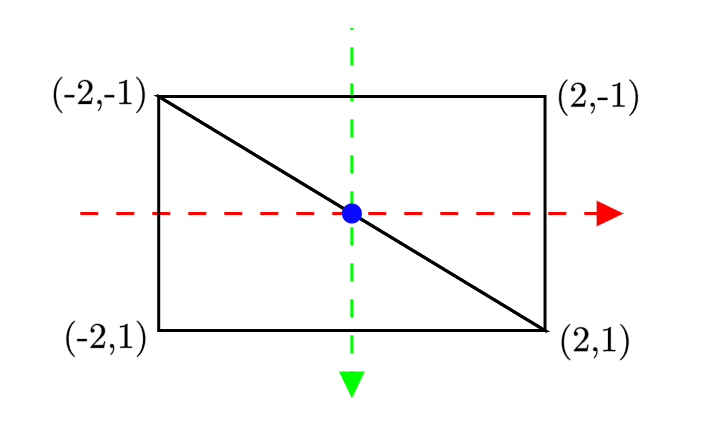
\includegraphics[width=\textwidth]{canvas.png}
    \end{minipage}
    \caption{Declaración de vértices del lienzo}
    \label{fig:canvas}
\end{figure}
Observamos en la \autoref{fig:vert} que como necesitamos dos triángulos, y por tanto dos grupos de tres vértices, hemos tenido que repetir dos vértices. Para formar los triángulos hacemos uso del método \texttt{gl.drawArrays}, el cual renderiza primitivas a partir de un array de datos. Como queremos dibujar triángulos, la primitiva será \texttt{GL\_TRIANGLES}. Al indicar esta primitiva, se tomarán los vértices del búfer de tres en tres y se dibujará un triángulo con ellos, así que es imprescindible que el orden en el que los hayamos definido sea el correcto. Adicionalmente, indicamos que el índice de inicio es el primero y que use los seis vértices definidos con los parámetros \texttt{offset} y \texttt{count} respectivamente.
\begin{lstlisting}[language=JavaScript]
function drawScene() {
  var primitiveType = gl.TRIANGLES;
  var offset = 0;
  var count = 6;
  gl.drawArrays(primitiveType, offset, count);
}
\end{lstlisting}
Una vez definida la geometría, quedaría escribir el \textit{vertex shader}, para el cual recordemos que tendríamos que calcular las matrices de transformación necesarias. Sin embargo, dado que \texttt{WebGL} es una API en 2D, solo necesitamos pasar directamente de coordenadas locales a recortadas, y este cálculo nos lo proporciona \texttt{WebGL} a través del método \texttt{gl.getAttribLocation}. Juntando esto con lo explicado para la definición de triángulos, obtendríamos que un escenario mínimo de uso de \texttt{WebGL} es el siguiente \cite{webgl_ejemplo}.
\begin{lstlisting}[language=JavaScript]
// Crear contexto WebGL
var canvas = document.getElementById("canvas");
var gl = canvas.getContext("experimental-webgl");

// Crear y asignar shaders
var vertexShader = createShaderFromScriptElement(gl, "2d-vertex-shader");
var fragmentShader = createShaderFromScriptElement(gl, "2d-fragment-shader");
var program = createProgram(gl, [vertexShader, fragmentShader]);
gl.useProgram(program);

// Coordenadas recortadas
var positionLocation = gl.getAttribLocation(program, "u_position");

// Declaración de vertices
var buffer = gl.createBuffer();
gl.bindBuffer(gl.ARRAY_BUFFER, buffer);
gl.bufferData(
    gl.ARRAY_BUFFER,
    new Float32Array([
      -2, -1,
       2, -1,
      -2,  1,
       2, -1,
      -2,  1,
       2,  1]),
    gl.STATIC_DRAW);
    
gl.enableVertexAttribArray(positionLocation);
gl.vertexAttribPointer(positionLocation, 2, gl.FLOAT, false, 0, 0);

// Dibujar lienzo
gl.drawArrays(gl.TRIANGLES, 0, 6);
\end{lstlisting}
El \textit{vertex shader} será tan sencillo como
\begin{lstlisting}
uniform vec2 u_position;

void main() {
  gl_Position = vec4(u_position, 0, 1);
}
\end{lstlisting}

% Pasamos ahora a estudiar el \textit{fragment shader}. 

% Los atributos que usaremos son los que siguen.
% \begin{itemize}
%     \item \textbf{\texttt{in vec4 gl\_FragCoord}}: coordenadas de dispositivo para el centro del píxel actual en el \textit{fragment shader}. Al ser un atributo de entrada del \textit{fragment shader}, está interpolada en cada vértice. La cuarta componente es la inversa de la componente homogénea de \texttt{gl\_Position}, y se utiliza en el cálculo de la profundidad de los píxeles y en las operaciones de corrección de perspectiva. 
%     \item \textbf{\texttt{out vec4 gl\_FragColor}}: terna RGBA para asignar el color del píxel actual en el \textit{fragment shader}.
% \end{itemize}
% Como sabemos, se ejecutará una instancia del \textit{fragment shader} por cada píxel en pantalla, y el objetivo de cada una de ellas será el de asignar un color a su píxel a través de \texttt{gl\_FragColor}. 

Pasamos ahora a estudiar el \textbf{\textit{fragment shader}}. Dado que el código es el mismo usemos \texttt{WebGL} o React, vamos a ver cómo lo hemos implementado en el contexto de nuestra aplicación de React, ya que este tiene la particularidad de que tendremos que pasárselo a \texttt{gl-react} en forma de \texttt{string}. Gran parte de su contenido es estático, incluyendo las constantes usadas en el algoritmo de \textit{spheretracing} (iteraciones máximas, precisión, distancia dibujado) o el código de los operadores vistos en la \autoref{sec:operaciones} y los algoritmos de cálculo de iluminación, oclusión ambiental y \textit{antialiasing}. Esto hace que el \textit{shader} puede estar definido en un archivo a parte como una función que recibe una serie de parámetros y devuelve una cadena de texto. Sin embargo, hay elementos del \textit{shader} que son dinámicos debido a que el usuario puede modificarlos de una forma u otra. Estos serán pasados como \texttt{props} al componente de lienzo, que a su vez los pasará al \textit{fragment shader} cuando detecte un cambio en alguno de ellos.
\begin{lstlisting}[language=JavaScript, caption=Definición del procesador de fragmentos]
export const fs = (sdf, primitives, aa, ao, shadow) => {
    return `
        // fragment shader ...
    `
}
\end{lstlisting}

El  más importante de los argumentos recibidos por el componente es la propia función distancia con signo en forma de cadena de texto, cuyo valor cambia tras prácticamente cada acción del usuario tanto en el editor de nodos como en el panel de primitivas que estudiaremos más adelante. Lo ideal sería pasar todos los parámetros al \textit{shader} a través de \textit{uniforms}, pero estos no pueden ser del tipo \texttt{string}, lo que hace imposible usarlos para la función distancia. En su lugar, no tenemos más remedio que recompilar el \textit{shader} cada vez que se modifica la función distancia, siendo este el mayor cuello de botella de la aplicación. Para modificar la menor cantidad de código, existe una función predefinida \texttt{sdf} vacía en el \textit{shader}, que recibe un punto $p$ y devolverá la expresión evaluada por GLSL de la función distancia en dicho punto, siendo esta la equivalente a la función distancia con signo $\phi$ del \autoref{alg:fsFinal}. Además, dado que al usuario se le permitirá usar directamente las variables $x,y,z$ al introducir una función distancia con signo en lugar de tener que escribir \texttt{p.x} o \texttt{p[0]} para acceder a las componentes del punto \texttt{p}, estas se declaran previamente con los nombres \texttt{x}, \texttt{y}, \texttt{z}. Sin embargo, no será esta función \texttt{sdf} la que evalúen todos los algoritmos de renderizado para sus cálculos, sino la función \texttt{map}, que devuelve una estructura del tipo \texttt{Surface} conteniendo la distancia con signo a la superficie desde el punto actual y el material que tiene asignado la superficie. A su vez, este material viene representado por la estructura \texttt{Material}, que encapsula los atributos de reflexión difusa, especular, ambiental, etc. La razón de usar esta función es que se pueda trabajar con varias superficies al mismo tiempo, cada una con un material, lo cual permite un mayor grado de control sobre el aspecto de la escena y, por ejemplo, ser capaz de interpolar los materiales de dos superficies al realizar operaciones booleanas, como se mostró en la \autoref{fig:smoothVS}.\newline

Otro factor cambiante en el \textit{fragment shader} son las primitivas disponibles, ya que el usuario podrá crear nuevas superficies a partir de ellas, y por tanto deberán estar declaradas en el \textit{shader}. Al igual que antes, deberemos recompilar el \textit{shader} cada vez que se realice un cambio sobre las primitivas almacenadas, del cual nos notificará el \textit{hook} del contenedor de Zustand, ya que tendremos que modificar el código fuente del \textit{shader}. Cada primitiva tendrá asignada una función en el \textit{shader}, recibiendo el punto \texttt{p} en el que ser evaluada y un argumento por cada parámetro de la primitiva. Así, cuando se detecte un cambio se generará una cadena de texto con la definición de todas las primitivas, que la función \texttt{fs} recibirá como argumento e insertará en el código del \textit{shader}.\newline
\begin{lstlisting}[language=JavaScript, caption=Ejemplo de declaración de primitiva]
float Sphere(vec3 p, float radius){
    return length(p) - r;
}
\end{lstlisting}
Resulta también interesante permitir al usuario elegit qué técnicas y algoritmos quiere utilizar para el renderizado, y que así pueda apreciar las diferencias en tiempo real. En nuestro caso definiremos directivas asociadas a los algoritmos de sombras y oclusión ambiental, así como al factor de escalado del \textit{antialiasing}, con lo que conseguimos que solo esté presente el código de los algoritmos que se vayan a utilizar en el momento de la compilación. En el caso de los algoritmos de cálculo de sombras y oclusión ambiental, estos están definidos en funciones independientes que devuelven un factor de intensidad del efecto que será usado por el método que calcula la iluminación. En el caso del \textit{antialiasing} lo que cambia no es la presencia o ausencia de una función, sino la estructura del \texttt{main}, ya que es ahí donde se realiza el doble bucle necesario para aumentar la resolución de muestreo. En caso de que se tome \texttt{AA = 1}, este bucle no formará parte del código del \texttt{main}.\newline

El resto de parámetros variables del \textit{shader} se pueden pasar mediante \textit{uniforms}, pues son del tipo \texttt{float} o \texttt{float[]}, e incluyen:
\begin{itemize}
    \item Material de la primitiva con la estructura mostrada en la \autoref{fig:contenedorPrim} a través de varios \texttt{vec3} y \texttt{float}. 
    \item Resolución del lienzo en píxeles como un \texttt{vec2}, pasada desde el componente de React.
    \item La dirección, color y tamaño de las luces como \texttt{float[]}, agrupados de tres en tres en el caso de la dirección y el color. Dado que GLSL solo admite arrays de longitud fija, se ha fijado el número de luces en cuatro, aunque por defecto solo se utilizan dos, al igual que en el ejemplo de la \autoref{sec:ilum},
    \item Dos ángulos como un \texttt{vec2} y una distancia como \texttt{float} actuando como coordenadas esféricas del observador respecto al origen. Ambos parámetros se controlan por el usuario a través del ratón y se utilizan para obtener la matriz de cámara presentada en la ecuación \eqref{eq:rayo}.
\end{itemize}
A continuación se presenta el contenido básico del \textit{frament shader} coloreado según la sintaxis GLSL, pero recordar que en realidad lo que se devuelve es una cadena de texto.
\begin{lstlisting}[language=GLSL, caption=Procesador de fragmentos]
${ao==true ? "#define AO" : ""}
${shadow==true ? "#define SHADOWS" : ""}  
#define AA ${aa}

// Constants
const int MAX_MARCHING_STEPS=255;
const float MIN_DIST=0.;
const float MAX_DIST=100.;
const float PRECISION=.0001;
const float EPSILON=.0005;
const float PI=3.14159265359;

// Uniforms
uniform vec2  u_resolution;
uniform vec3  u_ambient;
// ...

float sdf(vec3 p){
    float x = p.x;
    float y = p.y;
    float z = p.z;
  
    return ${sdf};
}

struct Material
{
  vec3 ambient;   float ka;
  vec3 diffuse;   float kd;
  vec3 specular;  float ks;
  vec3 emission;
  float smoothness;
};

struct Surface{
  float sd;
  Material mat;
};

// == OPERATORS ==
float Union(float a,float b,float k,float n,out float interp){
  if(k==0.)
    return min(a,b);
  
  float h=max(k-abs(a-b),0.)/k;
  float m=pow(h,n)*.5;
  float s=m*k/n;
  
  interp=a<b?m:1.-m;
  return(a<b)?a-s:b-s;
}

vec3 Twist(in vec3 p,in float k){
  float c=cos(k*p.y);
  float s=sin(k*p.y);
  mat2 m=mat2(c,-s,s,c);
  vec3 q=vec3(m*p.xz,p.y);
  return q;
}

vec3 InfiniteRepeat(in vec3 p,in float s){
  return mod(p+.5*s,s)-.5*s;
}

// ...

// == USER PRIMITIVES ==
${primitives}$

// == SDF ==
float sdf(vec3 p){
  float x = p.x;
  float y = p.y;
  float z = p.z;
  float interp;
  
  return ${sdf};
}

Surface map(vec3 p){
  Material mat = Material(
    u_ambient,    // ambient
    u_ka,         // ka
    u_diffuse,    // diffuse
    u_kd,         // kd
    u_specular,   // specular
    u_ks,         // ks
    u_emission,   // emission
    u_smoothness  // smoothness
  );
  float d = sdf(p);
  
  return Surface(d, mat);      
}

Surface rayMarch(vec3 ro,vec3 rd,float start,float end){
  float depth=start;
  Surface co;
  
  for(int i=0;i<MAX_MARCHING_STEPS;i++){
    vec3 p = ro + depth*rd;
    co=map(p);
    depth += co.sd;
    if(co.sd<PRECISION||depth>end)
        break;
  }
  
  co.sd=depth;
  
  return co;
}

// == ILUMINATION ==
vec3 lighting(vec3 pos, vec3 rd, vec3 nor, Surface s){
    vec3 result = u_ambientEnv + s.mat.emission;
    float occ = 1.0;
    
    #ifdef AO
    occ= calcAO(pos,nor);
    #endif

    for(int i=0; i<4; i++){ // Fijamos el maximo de luces en 4
      if(u_lightsEnable[i] > 0){ 
          vec3 Li = normalize(vec3(u_lightsPos[3*i], u_lightsPos[3*i+1], u_lightsPos[3*i+2]));
          vec3 lColor = vec3(u_lightsColor[3*i], u_lightsColor[3*i+1], u_lightsColor[3*i+2]);
          vec3 h = normalize(Li-rd);
          float NLi = max(0.,dot(nor,Li));
          float NH = max(0.,dot(nor,h));
    
          float shadow = 1.0;
          #ifdef SHADOWS
          shadow=calcSoftshadow(pos,Li,.02,2.5,u_lightsSize[i]);
          #endif
          vec3 amb = s.mat.ka*s.mat.ambient;
          vec3 dif = NLi*s.mat.kd*s.mat.diffuse;
          vec3 spe = NLi*s.mat.ks*s.mat.specular*pow(NH,s.mat.smoothness);
    
          spe*=.04+.96*pow(clamp(1.-dot(h,Li),0.,1.),5.);
          result += lColor*(amb+dif + spe)*occ*shadow;
      }
    }

    return result;
}

// == CAMERA MATRIX ==
mat3 camera(vec3 cameraPos,vec3 lookAtPoint){
  vec3 cd=normalize(lookAtPoint-cameraPos);
  vec3 cr=normalize(cross(vec3(0.,1.,0.),cd));
  vec3 cu=normalize(cross(cd,cr));
  
  return mat3(-cr,cu,-cd);
}

// == MAIN ==
void main()
{
  const vec3 backgroundColor=vec3(0.95);
  const vec3 lookAt=vec3(0.);

  vec3 col=vec3(0.);
  vec3 eye=vec3(3.,3.,5.);
  mat3 rot=(RotateY(u_cameraAng.x)*RotateX(u_cameraAng.y));
  eye=rot*eye*u_zoom;
  mat3 cam = camera(eye,lookAt);

  #if AA>1
    for( int m=0; m<AA; m++ )
    for( int n=0; n<AA; n++ )
    {
      vec2 o = vec2(float(m),float(n)) / float(AA) - vec2(0.25);
      vec2 uv=((gl_FragCoord.xy+o) - 0.5*u_resolution.xy) / u_resolution.y;
  # else
    vec2 uv = (gl_FragCoord.xy - 0.5*u_resolution.xy) / u_resolution.y;
  #endif
  
  vec3 rayDir=cam*normalize(vec3(uv,-1));
  Surface co=rayMarch(eye,rayDir,MIN_DIST,MAX_DIST);
  
  if(co.sd>MAX_DIST){
    col+=backgroundColor;
  }
  else{
    vec3 p=eye+rayDir*co.sd;
    vec3 normal=calcNormal(p);
    
    col += lighting(p, rayDir, normal, co);
  }
  
  #if AA>1
    }
    col /= float(AA*AA);
  #endif
  
  gl_FragColor=vec4(col,1.);
  return;
}
\end{lstlisting}


Como se comentó al principio de la sección, unos de los objetivos de la aplicación es que sea lo más accesible posible al usuario, siendo la detección y comunicación de errores esencial para ello. La elección de la librería \texttt{gl-react} fue en gran parte debida a que incorpora la posibilidad de instalar manejadores para multitud de eventos mediante la instalación de un centinela, o \texttt{Visitor}, siendo el que más nos interesa el de \texttt{onSurfaceDrawError}. Este nos permitirá  capturar y reaccionar ante los fallos de compilación del \textit{shader}, así como acceder al mensaje de error. Este mensaje suele ser muy extenso, pero siempre tiene una estructura similar, de forma que podemos extraer la información útil para el usuario y mostrársela en tiempo real. Como ejemplo, observemos el siguiente error.
\begin{lstlisting}
exampleSDF(p,1.0000):  gl-shader: Error compiling vertex shader helloGL:
ERROR: 0:270: 'lengthh' : no matching overloaded function found

Error compiling vertex shader helloGL:
268:             float z = p.b;
269:       
270:             return lengthh(p) - r;
\end{lstlisting}
La información que interesa al usuario es la que está en la segunda línea. Con la expresión regular \texttt{/ERROR: \textbackslash d+:\textbackslash d+:(.*)/} podemos buscar el patrón \texttt{ERROR:} seguido de dos grupos de uno o más dígitos (\texttt{(\textbackslash d+)}) separados por dos puntos . Luego, nos quedamos con el texto que aparezca después del patrón hasta el final de la línea con \texttt{(.+)}, obteniendo el mensaje que queríamos.\newline

Teniendo en cuenta todo lo explicado anteriormente, ya podemos entender la estructura básica del componente \texttt{Lienzo}.
\begin{lstlisting}[language=JavaScript, caption=Componente del lienzo]
    // Importar fragment shader
    import { fs } from "./fragmentShader"; 
    
    // Obtener las funciones de las primitivas del contenedor de Zustand
    const selector = () => (store: any) => ({
        savedPrimitives: store.primitives.map((p: any) => `
            float ${p.fHeader}{
              float x = p.r;
              float y = p.g;
              float z = p.b;
            
              return ${p.parsedInput};
            }\n`
        ).join("\n"),
    });
    
    
    function Lienzo(props: {
      sdf: string;
      primitives: string;
      width: number | null;
      height: number | null;
      onError?: (e: string) => void;
      uniforms?: any[];
      material: Material;
    }) {
        const { savedPrimitives } = usePrimitiveStore(selector(), shallow);
        const [compileError, setCompileError] = useState(false);
        const [errorMsg, setErrorMsg] = useState("");
        const [shader, setShader] = useState<ShaderIdentifier>(defaultShader);
        // ... Otras variables ...
        const visitor = new Visitor();  // Centinela de gl-react
    
        // Manejador de error de compilacion del shader
        visitor.onSurfaceDrawError = (e: Error) => {
          if (props.onError) props.onError(e.message);
          console.warn(`ERROR COMPILING SHADER ${props.sdf}: `, e.message);
          setCompileError(true);
          setErrorMsg(e.message);
          return true;
        };
    
        // Recompilar cuando recibimos nuevo SDF o primitivas
        useEffect(() => {
            if(props.sdf === ""){
              setCompileError(true);
              return;
            }
            
            setCompileError(false);
            setShader(fs(props.sdf, props.primitives));
        }, [props.sdf, props.primitives]);
    
        // ... mouse handlers here ...
        
        return (
        <div>
            <Surface
                visitor={visitor}
                width={props.width || 100}
                height={props.height || 100}
            >
            <Node
              shader={shader}
              uniforms={{
                u_specular, u_diffuse, u_smoothness, u_emission,
                u_ka, u_ks, u_kd,
                u_ambientEnv, u_ambient,
                u_cameraAng, u_zoom,
                u_resolution,
                u_lightsPos, u_lightsColor, u_lightsSize
              }}
            />
          </Surface>
        </div>)
    }
    
    export const Shader = memo(MyShader);    
\end{lstlisting}


\section{Editor de nodos}
Este componente se basa en React Flow \cite{react-flow}, una librería muy completa que permite la implementación de diagramas interactivos basados en nodos. Los nodos tienen puertos de entrada (solo permiten la conexión con un nodo) y salida (permiten conectarse a varios nodos), así como un cuerpo que representa su contenido mediante un componente de React o una expresión JSX. React Flow permite definir tipos de nodos según nuestras necesidades, que en nuestro caso usaremos para representar las primitivas y las operaciones que podemos realizar sobre ellas.\newline

La estructura de todos estos nodos es similar. Todos cuentan con un encabezado que muestra de qué tipo son, un desplegable para elegir la primitiva u operación a usar seguido de un área con controles para los parámetros que estas puedan tener, un lienzo para mostrar el resultado de las operaciones aplicadas hasta el momento, y un botón para contraer el nodo ocultando toda la información excepto el encabezado. Debido a esto, tiene sentido tener un componente nodo general que se pueda adaptar a diferentes tipos de uso. El encabezado y elementos del desplegable se pasan fácilmente a través de \texttt{props}. Sin embargo, los parámetros sí dependen fuertemente del tipo de nodo en particular, y serán implementados por cada tipo de nodo por separado y pasado al general a través del parámetro \texttt{children}.\newline

El \textbf{nodo de primitiva} es el más sencillo, y permite seleccionar una primitiva entre las guardadas para ser conectada a uno o varios nodos de operaciones. Dado que su única función es proporcionar una primitiva base sobre la que realizar operaciones, no tiene ningún puerto de entrada. En su cuerpo podremos encontrar los controles para elegir la primitiva y modificar los posibles parámetros de esta, así como un lienzo que muestra los cambios en tiempo real.\newline

Los \textbf{nodos de operaciones} implementan las operaciones explicadas en la \autoref{sec:operaciones} y las aplican a las primitivas que reciben por sus puertos de entrada. A su vez hay cuatro tipos diferentes de estos nodos, uno por cada tipo de operación. Los nodos de operaciones de transformación, deformación y repetición tienen un único puerto de entrada, pues son operadores unarios. El nodo booleano sin embargo es capaz de recibir un número arbitrario de primitivas, incrementando el número de puertos de entrada según se conecten nuevas primitivas. La razón de permitir más de dos primitivas de entrada cuando los operadores booleanos son binarios es que si se quiere realizar una misma operación de forma reiterada sobre varias primitivas se necesitarían crear muchos nodos. Trabajar con tantos nodos sería tedioso y haría mucho menos legible el editor. Así, si un nodo booleano recibe las primitivas $A_i$ con $i\in \{1,\dots, n\}$, irá aplicando la operación de forma sucesiva sobre el resultado anterior según el orden de conexión. Por ejemplo, para la unión tendríamos
\begin{equation*}
    \bigcup_{i=0}^n A_i = A_n\bigcup \Big(A_{n-1} \bigcup ( \cdots A_2 \bigcup A_1)\Big).
\end{equation*}
\begin{figure}[!h]
    \centering
    \begin{subfigure}[b]{0.31\textwidth}
        \centering
        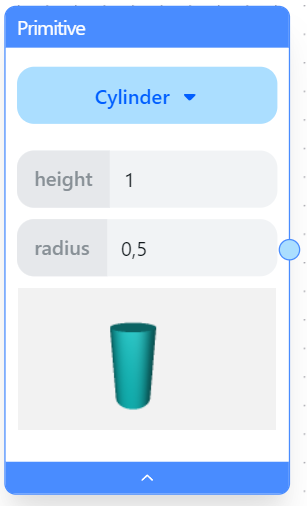
\includegraphics[width=\textwidth]{Plantilla-TFG-master/img/nodo_primitiva.png}
        \caption{Nodo de primitiva}
    \end{subfigure}
    \hspace{15pt}
    \begin{subfigure}[b]{0.32\textwidth}
        \centering
        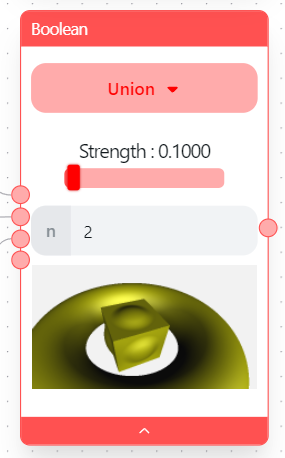
\includegraphics[width=\textwidth]{Plantilla-TFG-master/img/nodo_bool.png}
        \caption{Nodo de operador booleano}
    \end{subfigure}
    \hfill
    \caption{Ejemplos de tipos de nodos}
\end{figure}

De manera interna React Flow usa Zustand para almacenar la información relativa a los identificadores de los nodos, sus posiciones, conexiones, etc. Nosotros extenderemos esta funcionalidad para poder usar el modelo de generación de superficies en forma de árbol presentado en la \autoref{sec:operaciones}. Para ello bastará con almacenar para cada nodo la información relativa a su SDF actual, sus entradas y sus nodos hijos, así como funciones para gestionar los nodos (añadir, eliminar, actualizar, conectar, etc.). Mediante estas operaciones, cuando un nodo detecta una nueva conexión en algún puerto de entrada se leen las SDFs de todos ellos, y junto con los propios parámetros del nodo se actualiza la SDF del nodo. Cuando se elimina alguna conexión en el caso de los nodos diferentes al booleano simplemente la SDF pasa a ser indefinida. En el caso del booleano, habrá que tener en cuenta si todavía queda alguna entrada conectada, y en este caso reorganizar las restantes para que no haya puertos vacíos distintos al último y reducir el número de puertos a uno menos. Para esto, se detecta la posición del puerto que se ha eliminado y se modifican las conexiones siguientes para cambiar su puerto al inmediatamente anterior.\newline
\begin{figure}[!h]
    \centering
    \begin{subfigure}[b]{0.45\textwidth}
        \centering
        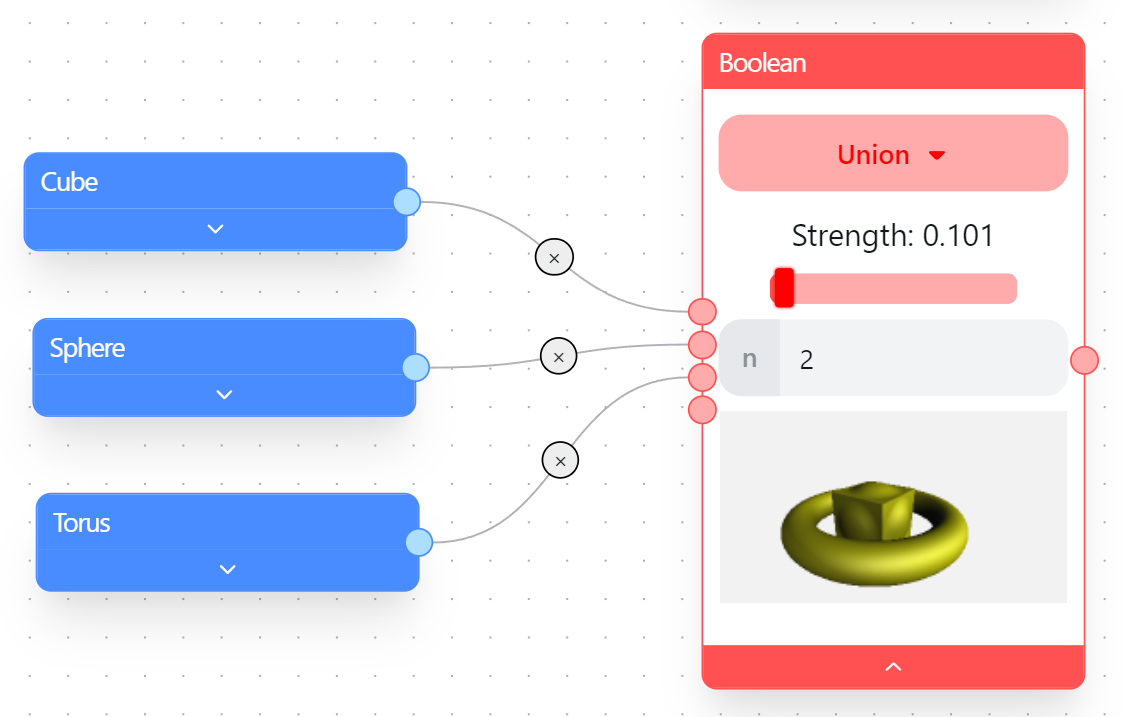
\includegraphics[width=\textwidth]{Plantilla-TFG-master/img/booleanBorrar1.png}
        \caption{Antes de eliminar}
    \end{subfigure}
    \hspace{15pt}
    \begin{subfigure}[b]{0.45\textwidth}
        \centering
        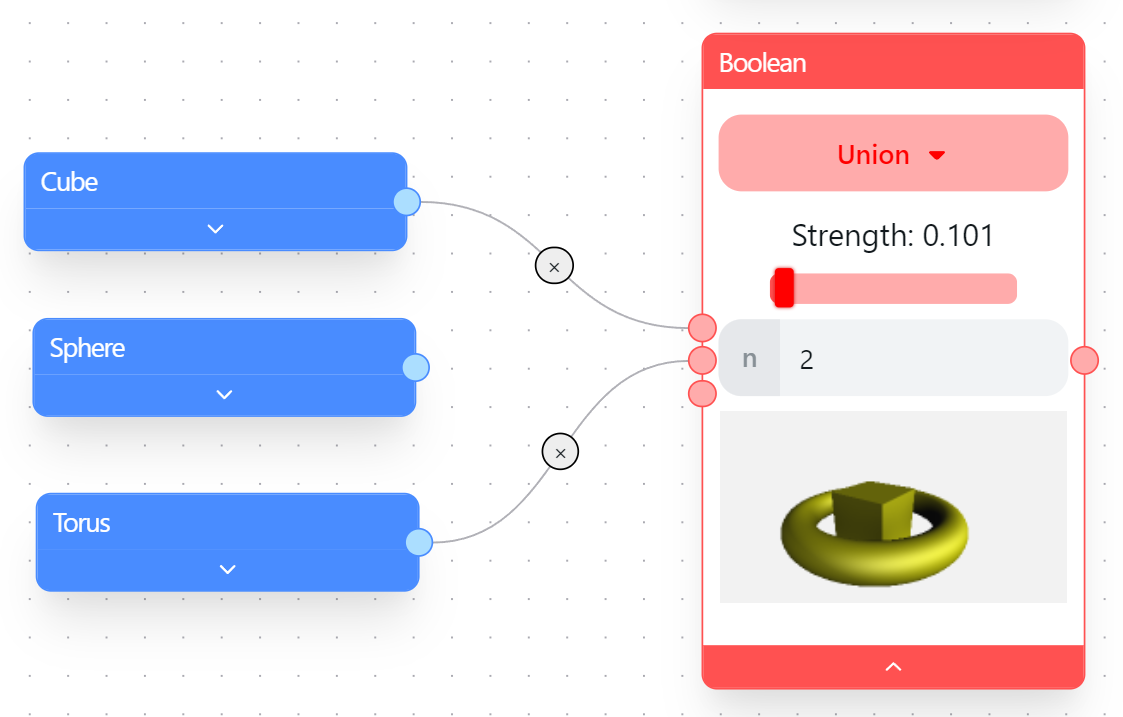
\includegraphics[width=\textwidth]{Plantilla-TFG-master/img/booleanBorrar2.png}
        \caption{Tras eliminar segunda conexión}
    \end{subfigure}
    \hfill
     \caption{Ejemplo de eliminación de conexión en nodo booleano}
\end{figure}

Terminamos realizando un ejemplo clásico de geometría de solidos constructiva haciendo uso del editor de nodos en la \autoref{fig:csg}.
\begin{figure}[ht!]
    \centering
    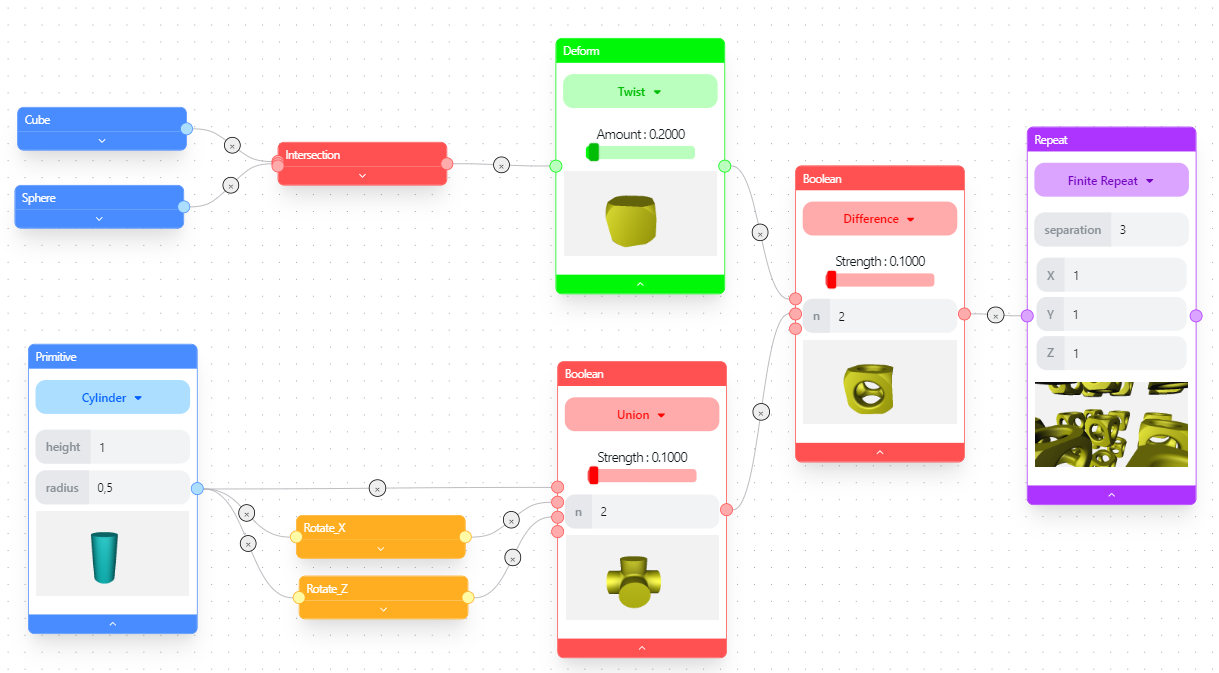
\includegraphics[width=\textwidth]{Plantilla-TFG-master/img/ejemploCSG.png}
    \caption{Ejemplo de CSG}
    \label{fig:csg}
\end{figure}

\section{Librería de polinomios en varias variables}
Para permitir al usuario definir superficies mediante ecuaciones paramétricas debemos de tener una forma de trabajar con polinomios en varias variables, y así poder aplicar el \autoref{t:implicitRac}. Si bien tenemos a nuestra disposición un gran número de librerías externas, en el momento de realización de la aplicación no se encontró ninguna opción viable para trabajar con este tipo de polinomios en JavaScript de forma nativa. Como alternativas se barajó el uso de la API de Geogebra \cite{geogebra} o realizar llamadas a código Python que usara SageMath \cite{sage}. Sin embargo, por motivos de rendimiento y completitud de este trabajo, se decidió desarrollar una librería nativa en TypeScript para el manejo de polinomios en varias variables, cálculo de bases de Gröbner e implicitación bajo el nombre de \texttt{multivariate-polynomial}. El código completo se encuentra disponible en \href{https://github.com/Daniel2000815/multivariate-polynomial}{https://github.com/Daniel2000815/multivariate-polynomial}, junto a su documentación, ejemplos de uso y tests usados. La librería consta de tres clases principales, cuya estructura se muestra en la \autoref{fig:clasesPol} y pasamos a estudiar a continuación en detalle.
\begin{figure}[ht!]
    \centering
    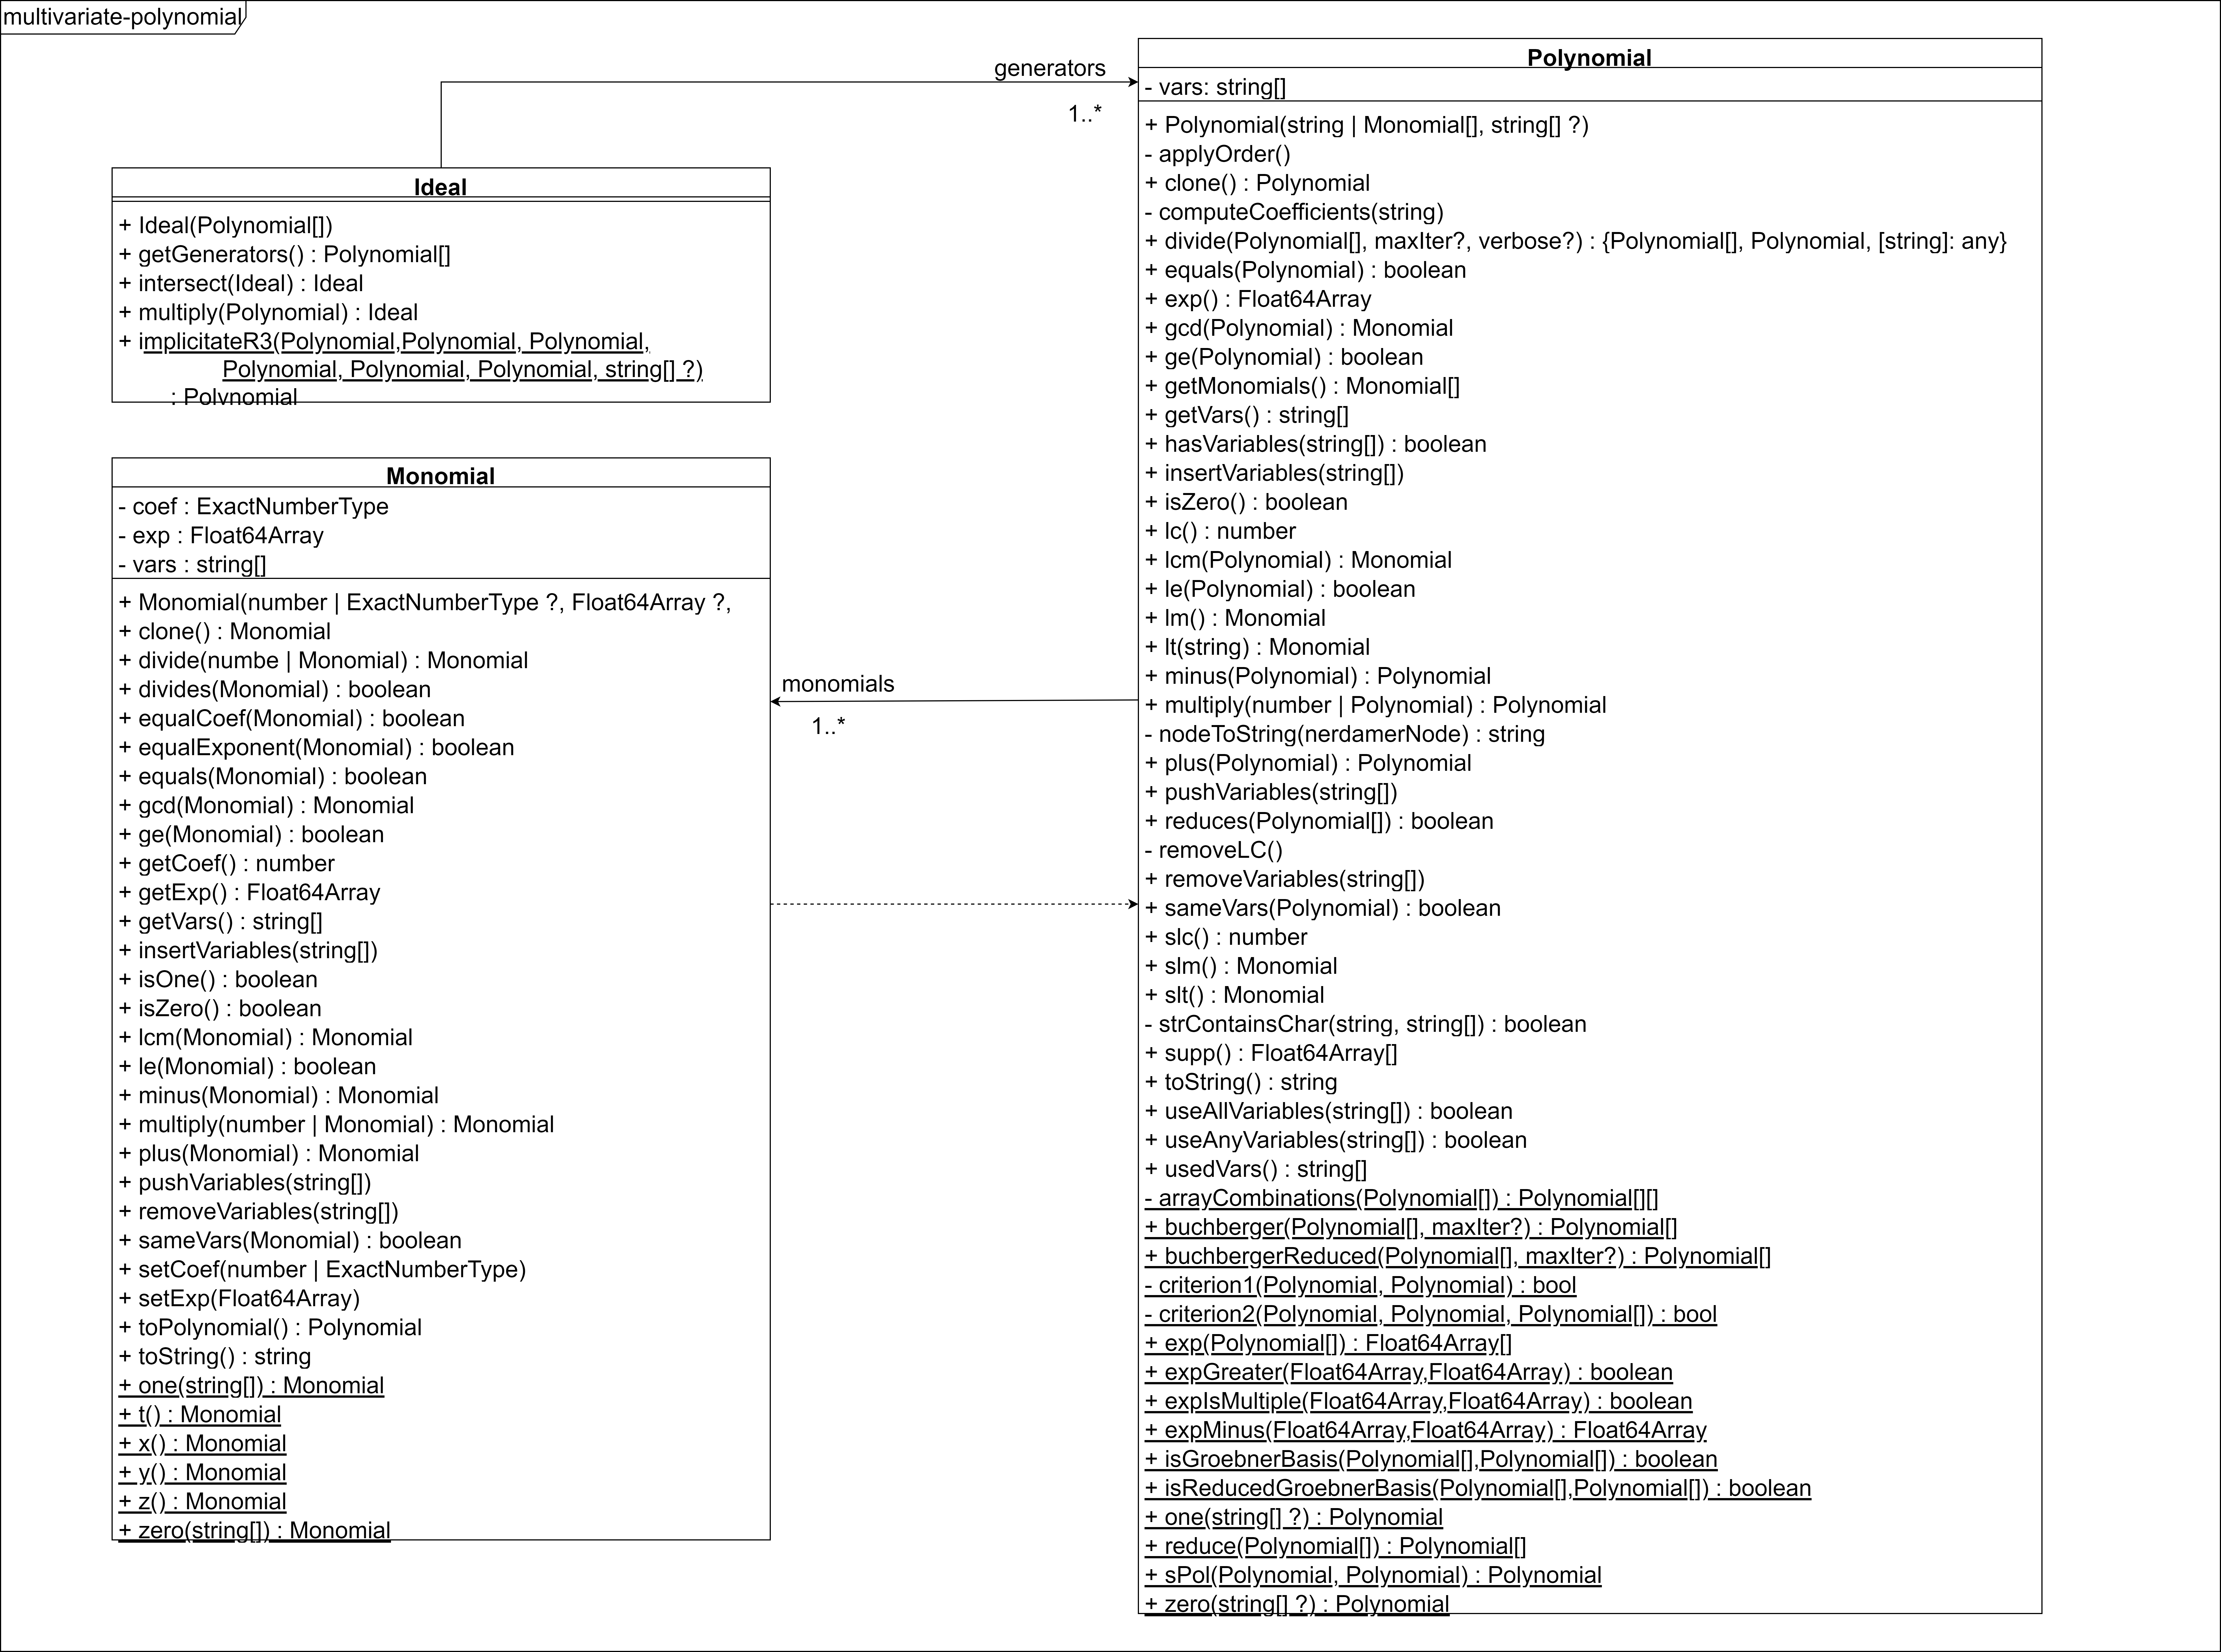
\includegraphics[width=\textwidth]{Plantilla-TFG-master/img/clasesPol.png}
    \caption{Diagrama de clases de la librería \texttt{multivariate-polynomial}}
    \label{fig:clasesPol}
\end{figure}

\subsection{Clase \texttt{Monomial}}
Representa un monomio en varias variables a través de los siguientes tres atributos.
\begin{itemize}
    \item \texttt{coef}: el coeficiente del monomio. En la primera versión implementada, este atributo estaba representado mediante el tipo primitivo de JavaScript \texttt{number}, el cual permite representar flotantes con una precisión similar al tipo \texttt{double} de Java o C\#. Esta elección hacía que en ocasiones hubiera errores en los cálculos debido a la falta de precisión que este tipo de representaciones acarrean, haciendo que por ejemplo al calcular una base de Gröbner no se pudieran reducir los términos líder correctamente. Por este motivo se decidió usar la librería \texttt{ExactNumber} \cite{ExactNumber}, la cual representa valores racionales como números decimales periódicos puros, permitiendo realizar operaciones elementales sin pérdida de precisión.
    \item \texttt{exp}: el exponente del monomio representado como un \texttt{Float64Array}, es decir, un array de flotantes de 64 bits. Se utilizó esta representación en lugar de un array convencional del tipo \texttt{number[]} debido a que al conocer de antemano el tamaño de los elementos del array (flotantes de 64 bits), tanto la escritura como la escritura son mucho más rápidas. Esto no ocurre con \texttt{number[]}, ya que \texttt{number} representa cualquier tipo de número.
    % como  la hora de realizar el cómputo de bases de Gröbner los valores de los exponentes pueden llegar a explotar, haciendo que no podamos continuar. Dado que el tipo \texttt{number} solo proporciona una precisión de 32 bits
    \item \texttt{vars}: variables del ideal al que pertenece el monomio representadas como \texttt{string[]}. El orden utilizado es \textit{lex} en función del orden que  ocupan las variables en el array.
\end{itemize}

El \textbf{constructor} de la clase tiene valores por defecto para cada atributo pudiendo el usuario indicar los que considere necesarios. El valor por defecto de los atributos son los del monomio nulo con variables usando las variables $t\le x\le y\le z$. Para comodidad del usuario, tanto en el constructor como en otros métodos se permite usar el tipo \texttt{number} y \texttt{number[]}, los cuales serán convertidos internamente al tipo \texttt{ExactNumberType} y \texttt{Float64Array} respectivamente. Además, se incluye un constructor de copia profunda y métodos estáticos para crear de forma rápida los monomios nulo, unidad, $t$, $x$, $y$ y $z$. Todos los atributos cuentan además con sus respectivos \textit{getters} y \textit{setters}.
\begin{lstlisting}[language=Javascript]
let m = new Monomial(2, [2,0,1,1], ["t", "x", "y", "z"])    // $2t^2yz en Q[t,x,y,z]$
let one = Monomial.one()
let x = Monomial.x()

let coef = x.getCoef() // 1
let exp = m.getExp()  // [2,0,1,1]
\end{lstlisting}

Las operaciones entre monomios son sencillas de implementar, pues solo requieren de manipulaciones básicas de los atributos \texttt{coef} y \texttt{exp}, junto a una comprobación de la igualdad del atributo \texttt{vars} para comprobar que trabajamos con monomios del mismo anillo. Dado que JavaScript no permite la sobrecarga de operadores, la única forma de usar las operaciones es a través de métodos de instancia que devuelvan un nuevo monomio. Se implementan las siguientes operaciones:
\begin{itemize}
    \item Suma: se suman los coeficientes tras comprobar que el exponente es el mismo.
    \item Multiplicación: se permite multiplicar tanto por un monomio como por un número. Si se pasa un número, bastará con multiplicarlo con el coeficiente del monomio. Si en su lugar se pasa un monomio se multiplican los coeficientes y se suman los exponentes componente a componente.
    \item Resta: se implementa como una suma junto a una multiplicación por $-1$ al segundo monomio.
    \item División: similar a la multiplicación, pero en su lugar los coeficientes se dividen y las componentes de los exponentes se restan. Antes de llevarla a cabo se debe comprobar que el monomio por el que se va a dividir es no nulo y cada componente de su exponente es menor a la del numerador.
    \item Igualdad: comprueba si tanto el coeficiente como el exponente de dos monomios coinciden.
    \item Orden: el método \texttt{le} implementa el orden \textit{lex} para comparar dos monomios, devolviendo \texttt{true} si el monomio actual es menor o igual que el pasado como argumento. Para ello se recorren simultáneamente las componentes de los exponentes de cada monomio hasta encontrar una posición en la que no coincidan. Se devolverá \texttt{true} si la entrada del monomio actual es menor a la del otro, y \texttt{false} en otro caso. Si ambos monomios tengan el mismo exponente se devuelve \texttt{true}. También existe el método \texttt{ge}, similar al anterior pero tomando como criterio si la entrada del exponente del monomio actual es mayor a la del otro.
    \item Mínimo común múltiplo: dado que estamos en $\Q$, el coeficiente del mínimo común múltiplo siempre será uno. En cuanto al exponente, basta con tomar el máximo de los exponentes de cada monomio en cada componente.
    \item Máximo común divisor: igual que el mínimo común múltiplo pero tomando el mínimo de las componentes de los exponentes.
\end{itemize}
\begin{lstlisting}[language=Javascript]
var resta = m.minus(one)            // 2t^2yz - 1
var mult  = m.multiply(x)           // 2t^2xyz
var div   = m.divide(Monomial.t())  // 2tyz
var lcm   = m.lcm(x)                // t^2xyz
\end{lstlisting}

Existe una para la restricción de JavaScript sobre no permitir la sobrecarga de operadores: el método \texttt{toString()}, el cual devuelve una representación como \textbf{cadena de texto} de la instancia de la clase. Que el usuario obtenga una representación clara y concisa del monomio será esencial para su experiencia con la librería. Para ello tendremos en cuenta varias cosas, como que si el coeficiente es positivo su signo se sobreentiende, y si es uno o menos este puede ser omitido. En cuanto a las variables comprobaremos si el valor de cada una en el exponente es cero, en cuyo caso no debe ser mostrada, o si es uno y no es necesario indicar la potencia.\newline

Por último, otros métodos de interés son los que permiten modificar las variables del anillo del monomio u obtener una instancia de un polinomio formado por el monomio en cuestión. También existen funciones para realizar diferentes comprobaciones sobre uno o varios monomios. Estas son usadas internamente para realizar comprobaciones previas antes de realizar determinadas operaciones, pero también están a disposición del usuario. Ejemplos de estas comprobaciones son si un monomio es nulo, si uno divide a otro, dos tienen el mismo exponente, mismas variables, etc.
\begin{lstlisting}[language=Javascript]
m.isZero()                  // false
m.divides(x)                // false
x.pushVariables(["w"]       // x.getVars() -> ["t","x","y","z","w"]
x.insertVariables(["s"]     // x.getVars() -> ["s","t","x","y","z","w"]
\end{lstlisting}
\subsection{Clase \texttt{Polynomial}}
Siguiendo la \autoref{def:polMultVar}, podemos representar un polinomio como una colección de monomios, que representaremos mediante el atributo \texttt{monomials} del tipo \texttt{Monomial[]}. La posición de los monomios en el array será en todo momento siguiendo el orden \textit{lex} para así simplificar la implementación de los métodos de instancia. Al igual que con los monomios, tendremos un atributo \texttt{vars} indicando las variables del anillo al que pertenece el polinomio, que será el mismo que el de los monomios que lo conforman. Así, el constructor de la clase \texttt{Polynomial} recibirá una lista con las variables del anillo y otra con los monomios. Se comprobará que todos los monomios pertenecen al mismo anillo, en cuyo caso serán ordenados usando \textit{lex} y el atributo \texttt{vars} tomará el valor del atributo homónimo de cualquier monomio pasado como argumento. De no pasarse ningún monomio, el polinomio será inicializado con el monomio nulo y las variables $t\le x\le y \le z$.\newline

Además de inicializar un polinomio mediante una colección de monomios creados individualmente, se permite al usuario pasar una cadena de texto del polinomio que quiere crear. Dado que internamente necesitamos trabajar con una lista de monomios, tendremos que extraer los monomios de la expresión. Para ello empezaremos parseando el \texttt{string} a un formato estructurado usando la librería de cálculo simbólico Nerdamer \cite{nerdamer}. Esta librería nos permite trabajar con los polinomios de manera básica, pero operaciones más avanzadas como el algoritmo de división no pueden ser implementadas, entre otros motivos porque Nerdamer no es compatible con el uso de órdenes monomiales. Nerdamer simplifica por defecto la expresión del polinomio que le pasemos, lo cual nos interesa, pero lo devuelve como producto de sus raíces. Podemos cambiar este comportamiento y hacer que nos lo muestre como una suma de monomios través del método \texttt{expand()}. Esto nos será necesario para continuar con el procedimiento de conversión del polinomio a nuestro formato. Tras esto ya podemos obtener la representación en árbol con notación polaca inversa (RPN) de la expresión parseada usando el método \texttt{tree()}.\newline

Una vez obtenida la estructura de árbol es sencillo localizar los monomios, pues estos solo pueden estar separados por un símbolo de adición o sustracción. Así, recorriendo el árbol en preorden, cuando encontremos un nodo que no tenga ninguno de estos símbolos como descendiente, el subárbol del que es nodo raíz representará un monomio. Una vez localizado el nodo, podemos obtener la expresión del monomio recorriendo el subárbol de nuevo en preorden.\newline
\begin{figure}[ht!]
    \centering
    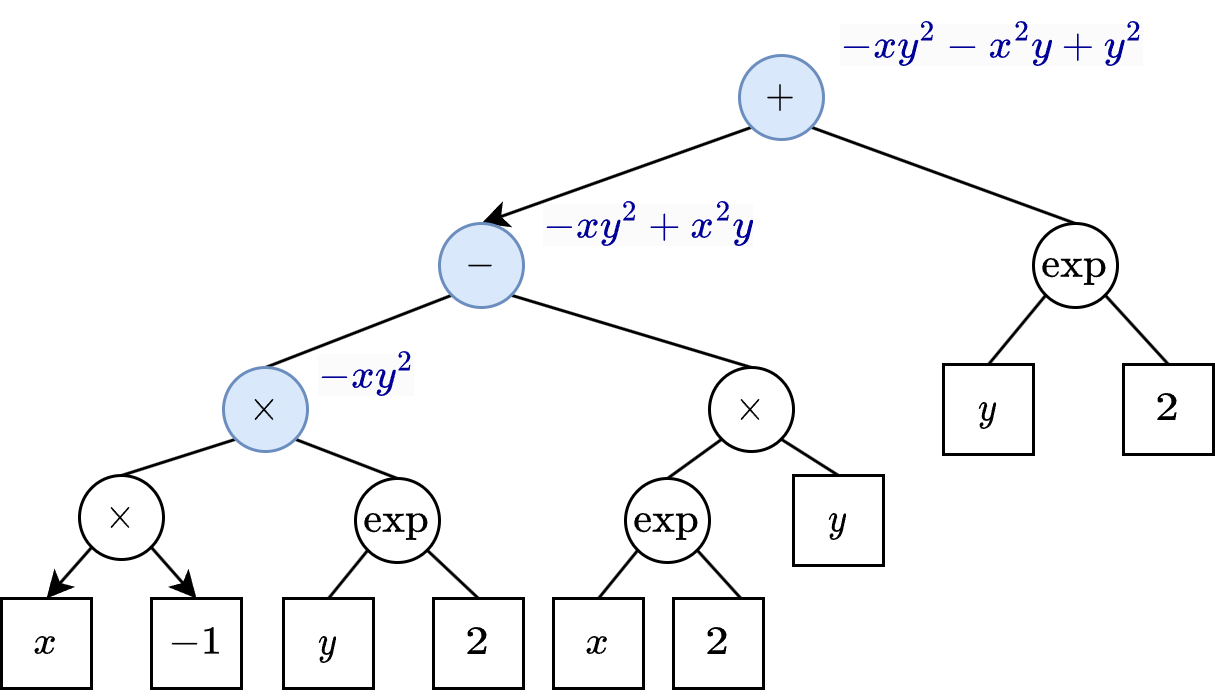
\includegraphics[width=0.85\textwidth]{Plantilla-TFG-master/img/busquedaMon.png}
    \caption{Ejemplo de búsqueda de monomios en el árbol}
    \label{fig:busquedaMonom}
\end{figure}

Dado que las variables del anillo siempre son pasadas al constructor del polinomio, solo necesitamos extraer el coeficiente y exponente de la expresión de cada monomio encontrado en el árbol. Como la expresión resultado de expandir cada nodo de un monomio siempre tendrá la forma \texttt{<coeficiente><variables>}, podemos simplemente recorrer la expresión hasta detectar un carácter no numérico, el cual marcará la división entre el coeficiente y las variables. Con esta información ya podemos crear la instancia de cada monomio que conforma al polinomio, pudiendo calcular su exponente de forma sencilla usando el método \texttt{deg} de Nerdamer, que nos proporciona el grado de la variable recibida como argumento de la expresión. A lo largo de este proceso tendremos que haber tenido cuidado de realizar varias comprobaciones de errores, como que se detecte alguna variable que no pertenece al anillo del polinomio, o casos especiales, como que el coeficiente sea uno o menos uno y no aparezca en la expresión. Como último paso deberemos aplicar el orden \textit{lex} a los monomios encontrados. La manera más sencilla es a través del método \texttt{sort} de JavaScript, el cual recibe un comparador binario como argumento. En nuestro caso este comparador será el de menor o igual ya implementado en la clase \texttt{Monomial}. Observamos que no puede ocurrir que dos monomios tengan el mismo exponente, ya que si no Nerdamer los habría simplificado en un único monomio.\newline

La implementación de la mayoría de las \textbf{operaciones básicas} es sencilla una vez se ha conseguido la representación como lista de monomios, pues muchas se basan en las operaciones ya implementadas para monomios.
\begin{itemize}
    \item Suma: para cada monomio se comprueban los siguientes de la lista cuyo exponente es el mismo mientras estos se van sumando y añadiendo a una lista auxiliar para asegurarnos de que no vuelvan a ser tenidos en cuenta. Si el monomio suma no es cero, se añade al polinomio resultado. Al igual que para los polinomios, se implementa la operación de resta a través de esta junto con un producto.
    \item Multiplicación: como en el caso de los monomios, este operador admite como parámetro tanto un \texttt{number} como una instancia de \texttt{Polynomial}. En el caso de que el argumento sea un escalar, solo hay que multiplicar cada monomio por él, teniendo en cuenta que si es cero podemos devolver directamente el polinomio nulo. En cuanto a la multiplicación por otro polinomio, hay que realizar un doble bucle multiplicando cada monomio de un polinomio por todos los del otro. En este proceso pueden generarse varios monomios con el mismo exponente aunque esto no ocurriese con los polinomios originales, como sería el caso de la multiplicación
    $$(xy - ty)\cdot(t+x) = \boldsymbol{txy} + x^2y -t^2y - \boldsymbol{txy} = x^2y -t^2y.$$
    Los monomios con mismo exponente serán por tanto sumados y añadidos al resultado si son distintos de cero.
    \item División: implementa el \autoref{a:division} haciendo uso de las operaciones de monomios y polinomios ya presentadas. Dado que esta operación puede llevar una cantidad considerable de tiempo, se puede indicar el máximo número de iteraciones a realizar, entendiendo como iteración el reducir el término líder del polinomio actual. Además, existe la posibilidad de obtener como resultado una lista con los pasos detallados seguidos para obtener el resultado mediante el parámetro \texttt{verbose}, aunque esta funcionalidad no está presente en la versión usada en la aplicación por motivos de eficiencia.
    \item Igualdad: comprueba si cada monomio de un polinomio está también en el otro. Dado que las entradas de \texttt{monomials} están ordenadas con \textit{lex} basta comparar cada componente del array.
    \item Orden: permite realizar las comparaciones $\le$ y $\ge$ sobre dos polinomios aplicando los métodos \texttt{le} y \texttt{ge} de la clase \texttt{Monomial} sobre los monomios líder de ambos polinomios.
    \item S-polinomio: implementado usando las operaciones resta y producto de polinomios y resta de exponentes (esta última no disponible para el usuario) tras comprobar que ambos polinomios pertenecen al mismo ideal. Es un método estático.
    \item Mínimo común múltiplo y máximo común divisor: usa los métodos de la clase \texttt{Monomial} sobre los exponentes de ambos polinomios.
\end{itemize}

Como no podía ser de otra forma, se incluyen \texttt{getters} para los atributos de la clase, así como métodos que nos permitan obtener información básica del polinomio de forma rápida, como \texttt{lm()} para el monomio líder, \texttt{sm()} para el segundo monomio líder, \texttt{supp()} para obtener el soporte del polinomio, etc. Gracias a la representación que hemos elegido, estos se basarán en aplicar consultas muy sencillas sobre los atributos de la clase. Otros métodos muy útiles son los que comprueban propiedades del polinomio, como si este reduce a cero sobre un conjunto de polinomios $F$ con \texttt{reduce(F)}.\newline

Esta clase también implementa su \textbf{representación como cadena de texto} basándose en la de la clase \texttt{Monomial}. En este caso se tienen en cuenta algunas consideraciones adicionales. Dado que cuando el coeficiente de un monomio era positivo no incluíamos el símbolo, no podemos simplemente concatenar las cadenas de texto de los monomios del polinomio, sino que habrá que comprobar para cada uno si debemos añadir nosotros el símbolo \texttt{+} como separador, a excepción de para el primero. También deberemos asegurarnos que el espaciado entre los monomios en consistente y se deja un espacio entre su símbolo y el resto de la expresión.\newline

Los métodos más importantes de esta clase son los relacionados con las \textbf{bases de Gröbner}, los cuales son estáticos. Se implementa el \autoref{a:buchberger} en el método \texttt{buchberger}, el cual recibe como argumento los generadores del ideal y opcionalmente un máximo de iteraciones. Este método hace un uso intensivo de los operadores de división y S-poliomio, así como la función \texttt{arrayCombinations} no accesible al usuario, que obtiene las parejas de polinomios que comparar siguiendo la estrategia normal. También hace uso de los criterios de Buchberger del \autoref{t:criterios}. Sus implementaciones son un buen ejemplo de como usar esta biblioteca de forma más avanzada, y a continuación mostramos la del segundo criterio.
\begin{lstlisting}[language=Javascript]
private static criterion2(f: Polynomial, g: Polynomial, G: Polynomial[]) : boolean {
    let res = false;
    const startIndex = Math.max(G.indexOf(f), G.indexOf(g)) + 1;

    for(let i=startIndex; i<G.length && !res; i++){
        const h = G[i];
        const sPolfh = Polynomial.sPol(f, h);
        const sPolgh = Polynomial.sPol(g, h);
    
        if(!h.lm().divides(f.lcm(g)))   continue;
        if(sPolfh.reduces(G) || sPolgh.reduces(G))  return true
        else{
          const lmH = h.lm();
          const gdcFG = f.gcd(g);
    
          const cond1 = lmH.divides(f.lm().divide(gdcFG)) && !g.slm().multiply(h.lm()).equals(h.slm().multiply(g.lm()));
          const cond2 = lmH.divides(g.lm().divide(gdcFG)) && !f.slm().multiply(h.lm()).equals(h.slm().multiply(f.lm()));
    
          res = cond1 || cond2;
        }
    }
    return res;
}
\end{lstlisting}
Para reducir la base obtenida se puede usar la función \texttt{reduce}, que asume que recibe una base de Gröbner y la reduce a través del \autoref{a:minim}. 
\begin{lstlisting}[language=Javascript]
static reduce(G: Polynomial[]) : Polynomial[]{
    let res : Polynomial[] = [];
    G = G.map(g => g.multiply(1/g.lc()));   // hacemos cada polinomio mónico (lc=1)

    for(let i=0; i<G.length; i++){
        let g = G[i];
        let div = g.divide(G.filter(e => !e.equals(g)));    // devuelve el resto y los coeficientes

        // si el resto no es cero, sustituimos el polinomio por el y lo añadimos a la base resultado 
        if(!div.remainder.isZero()){
            G[i] = div.remainder;
            res.push(div.remainder);
        }
    }
    return res;
}
\end{lstlisting}
Para obtener una base reducida directamente se puede usar \texttt{buchbergerReduced}, que ejecuta consecutivamente los métodos \texttt{buchberger} y \texttt{reduce}.
\begin{lstlisting}[language=Javascript]
static buchbergerReduced(F: Polynomial[], maxIter: number = 1000) {
    return this.reduce(this.buchberger(F, maxIter));
}
\end{lstlisting}

Por último, al igual que para la clase \texttt{Monomial}, se incluyen los métodos  \texttt{insertVariables}, \texttt{pushVariables} y \texttt{removeVariables} para añadir o eliminar variables del cuerpo del polinomio. Además, dado que para implementar el algoritmo de implicitación deberemos ser capaces de comprobar si un polinomio contiene ciertas variables, se ha implementado el método \texttt{useAnyVariables}, que recibe una lista de variables y comprueba si la entrada correspondiente en el exponente del polinomio de alguna de ellas es distinta de cero. También se puede usar \texttt{useAllVariables} para comprobar si se usan todas.

\subsection{Clase \texttt{Ideal}}
Esta clase consta de un único atributo, \texttt{gens}, representando una lista de los polinomios generadores del ideal. Los generadores son pasados como argumento al constructor, pero antes de asignar su valor a \texttt{gens} se calcula una base de Gröbner reducida suya para trabajar con el menor número posible de polinomios. Se incluyen los operadores de producto e intersección de ideales, que son muy sencillos de implementar usando los generadores. Sin embargo, el objetivo principal de esta librería era el de resolver el problema de implicitación de una parametrización racional. Usando bases de Gröbner habíamos llegado a la solución descrita \autoref{t:implicitRac}, y que implementamos en el método estático \texttt{implicitateR3} de esta clase. Como su nombre indica, se ha implementado para el caso $A^n = \R^3$ por motivos de eficiencia de la aplicación. Supondremos por tanto que la parametrización es de la forma
\begin{equation*}
    x = \frac{f_1(t_1,\dots, t_r)}{q_1(t_1,\dots, t_r)},\quad
    y = \frac{f_2(t_1,\dots, t_r)}{q_2(t_1,\dots, t_r)},\quad
    z = \frac{f_3(t_1,\dots, t_r)}{q_3(t_1,\dots, t_r)},
\end{equation*}
donde $f_1,f_2,f_3,q_1,q_2,q_3 \in \R[t_1,\dots, t_r]$ y $q_1,q_2,q_3 \neq 0$. A continuación estudiamos en detalle la implementación del algoritmo.\newline

La función recibe como argumentos las instancias de los polinomios $f_1,f_2,f_3,q_1,q_2,q_3$, comprobando que todos pertenecen al mismo cuerpo. En el caso de nuestra aplicación, esta creará estos polinomios según los datos que haya introducido el usuario, forzando a que este use las variables $s$ y $t$ para la parametrización. Sin embargo, la librería admite que se use cualquier combinación de variables a excepción de $x,y,z$, que están reservadas para las variables del ideal de eliminación del teorema. Si se detecta su uso, se generará una excepción. Por último, dado que en la aplicación el usuario es capaz de usar parámetros para modificar la superficie en el editor de nodos, estos deberán ser tratados como variables más del ideal de eliminación final, y se pueden pasar como parámetro opcional. Una vez identificadas las variables que ha usado el usuario, debemos buscar una más que no esté siendo usada para que asuma la función de la variable auxiliar $y$ del enunciado del teorema. Para ello basta con recorrer el alfabeto hasta encontrar un nombre libre para esta variable.\newline

Las comprobaciones anteriores nos permiten obtener los siguientes arrays de variables:
\begin{itemize}
    \item \texttt{elimVars}: son las variables $t_1,\dots, t_r,y$ del teorema, y no formarán parte del ideal resultado. En nuestro caso, serán las variables de los polinomios $f_1,f_2,f_3,q_1,q_2,q_3$ junto a la variable auxiliar obtenida previamente.
    \item \texttt{resVars}: variables $x_1,\dots, x_n$ del teorema. En nuestro caso serán $x,y,z$ y los parámetros usados por el usuario en la parametrización.
    \item \texttt{impVars}: variables del ideal $I$ del teorema, y por tanto las del cuerpo en el que trabajaremos durante el resto del algoritmo. Será la unión de los arrays anteriores. Dado que los polinomios $f_1,f_2,f_3,q_1,q_2,q_3$ pasados como argumento solo usan las variables en \texttt{elimVars}, el resto deberán ser añadidas con \texttt{pushVariables}.
\end{itemize}
Por ejemplo, en el caso de la parametrización del \autoref{ej:finalGroebner}, tendríamos
\begin{align*}
    f_1(s,t)&=&s+t&,\quad &f_2(s,t)&=&s&,\quad &f_3(s,t)&=&t,\\[7pt]
    q_1(s,t)&=&1&,\quad &q_2(s,t)&=&1&,\quad &q_3(s,t)&=&1,\\[7pt]
    \texttt{elimVars}&=&\texttt{[s,t]}&,\quad &\texttt{resVars}&=&\texttt{[x,y,z]}&,\quad &\texttt{elimVars}&=&\texttt{[s,t,x,y,z]}.
\end{align*}

Para obtener los generadores del ideal $I$, primero creamos polinomios para cada una de las variables $x,y,z$, además de la auxiliar. Estos pueden ser creados tanto pasando la cadena de texto con la variable como creando el exponente a mano. Por motivos de legibilidad, en este ejemplo elegimos la primera opción, aunque la segunda es más eficiente. Mediante operaciones de resta y producto obtenemos los generadores finales del ideal
$$I = \langle q_1x - f_1, q_2y - f_2, q_3z - f_3, 1 - q_1q_2q_3v_{aux}\rangle,$$
que son usados para crear una instancia de la clase \texttt{Ideal}. Una vez construido este ideal $I$, para obtener el ideal de eliminación $J$ basta con tomar los generadores de $I$ que no usen ninguna de las variables en \texttt{elimVars} mediante el método \texttt{useAnyVariables}. Si no se encuentra ningún generador, se devuelve el polinomio nulo, y si se obtiene más de uno se crea una excepción indicando que la parametrización no puede ser representada por una única ecuación implícita. En el mejor de los casos se obtendrá un único generador del ideal de eliminación, aunque este seguirá usando las variables de \texttt{elimVars}, lo cual no es deseable ni lo que el usuario espera, así que antes de devolverlo se eliminan esas variables del anillo del polinomio con \texttt{removeVariables}.\newline

El código final del algoritmo es el siguiente.
\begin{lstlisting}[language=JavaScript, caption=Algoritmo de implicitación]
static implicitateR3(fx: Polynomial, fy: Polynomial, fz: Polynomial, qx: Polynomial, qy: Polynomial, qz: Polynomial, parameters: string[] = []){
    if(!fx.sameVars(fy) || !fx.sameVars(fz) || !fx.sameVars(qx) || 
       !fx.sameVars(qy) || !fx.sameVars(qz))
      throw new Error("PARAMETRIZATIONS IN DIFFERENT RINGS");

    // Variables que ha usado el usuario en la parametrizacion distintas a x,y,z
    var elimVars = fx.getVars().filter(v => !parameters.includes(v));
    if(elimVars.some(v => ["x","y","z"].includes(v)))
      throw new Error("PARAMETRIZATIONS CAN'T USE X,Y,Z VARIABLES");

    // Buscamos variable auxiliar libre que despues sera eliminada
    const allVars = elimVars.join('');
    var variableAuxiliar = 'a';
    for (var letter of 'abcdefghijklmnopqrstuvw') {
      if (!allVars.includes(letter)) {
        variableAuxiliar = letter;
        break;
      }
      throw new Error("TOO MANY VARIABLES")
    }
    var posVarAux = elimVars.push(variableAuxiliar);
   
    // Variables del ideal J del teorema, parametros incluidos
    var resVars = parameters.concat(["x","y","z"]);

    // Variables del ideal I del teorema
    const impVars = elimVars.concat(resVars);

    // Construimos generadores de I
    const x = new Polynomial("x", impVars);
    const y = new Polynomial("y", impVars);
    const z = new Polynomial("z", impVars);
    const varAuxPol = new Polynomial(variableAuxiliar, impVars);

    const variablesToAdd = [variableAuxiliar].concat(resVars);
    fx.pushVariables(variablesToAdd); qx.pushVariables(variablesToAdd);
    fy.pushVariables(variablesToAdd); qy.pushVariables(variablesToAdd);
    fz.pushVariables(variablesToAdd); qz.pushVariables(variablesToAdd);
    const prod = Polynomial.one(impVars).multiply(qx).multiply(qy).multiply(qz).multiply(varAuxPol);
    const I = new Ideal([x.minus(fx), y.minus(fy), z.minus(fz), prod].concat());

    // Los generadores de J son los de I que contengan solo las variables de resVars
    var J : Polynomial[] = [];
    I.getGenerators().forEach(gen => {
      if(!gen.useAnyVariables(elimVars)){
        J.push(gen);
      }
    })

    if(J.length == 0)   
        return Polynomial.zero(resVars);
    else if(J.length ==1){
      var intersection = J[0];
      intersection.removeVariables(elimVars);
      return intersection;
    }
    else
      throw new Error("PARAMETRIZATION DOES NOT SATISFY AN UNIQUE IMPLICIT EQUATION");
  }
\end{lstlisting}








\section{Panel de primitivas}
En esta sección el usuario será capaz de visualizar y modificar las primitivas existentes, así como crear nuevas. Para ello se presenta una tabla que muestra la información más relevante de las primitivas presentes en el contenedor de Zustand, incluyendo en cada fila botones para editar o eliminar cada primitiva. 
\begin{figure}[ht!]
    \centering
    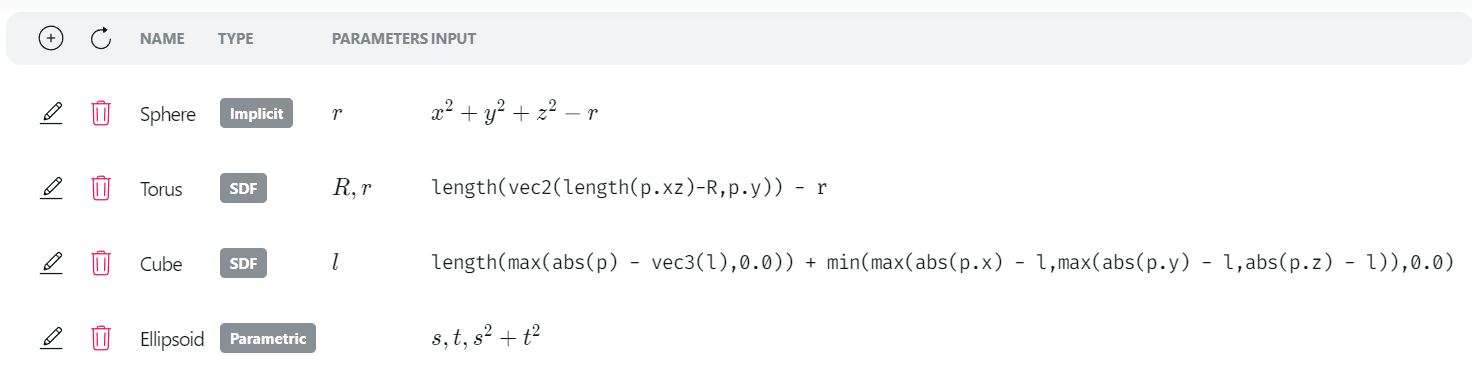
\includegraphics[width=\textwidth]{Plantilla-TFG-master/img/tablaParam.png}
    \caption{Tabla de primitivas}
\end{figure}

En el caso de que se desee eliminar alguna, bastará con llamar a la función correspondiente del contenedor. Si en cambio se desea realizar una modificación, se abrirá un cuadro de diálogo con toda la información de la primitiva, incluyendo los parámetros y ecuaciones que introdujo el usuario en el momento de la creación (razón por la cual guardábamos esta información en el contenedor) y el método de definición de la superficie (a través de una ecuación implícita, parametrización o SDF).\newline
\begin{figure}[ht!]
    \centering
    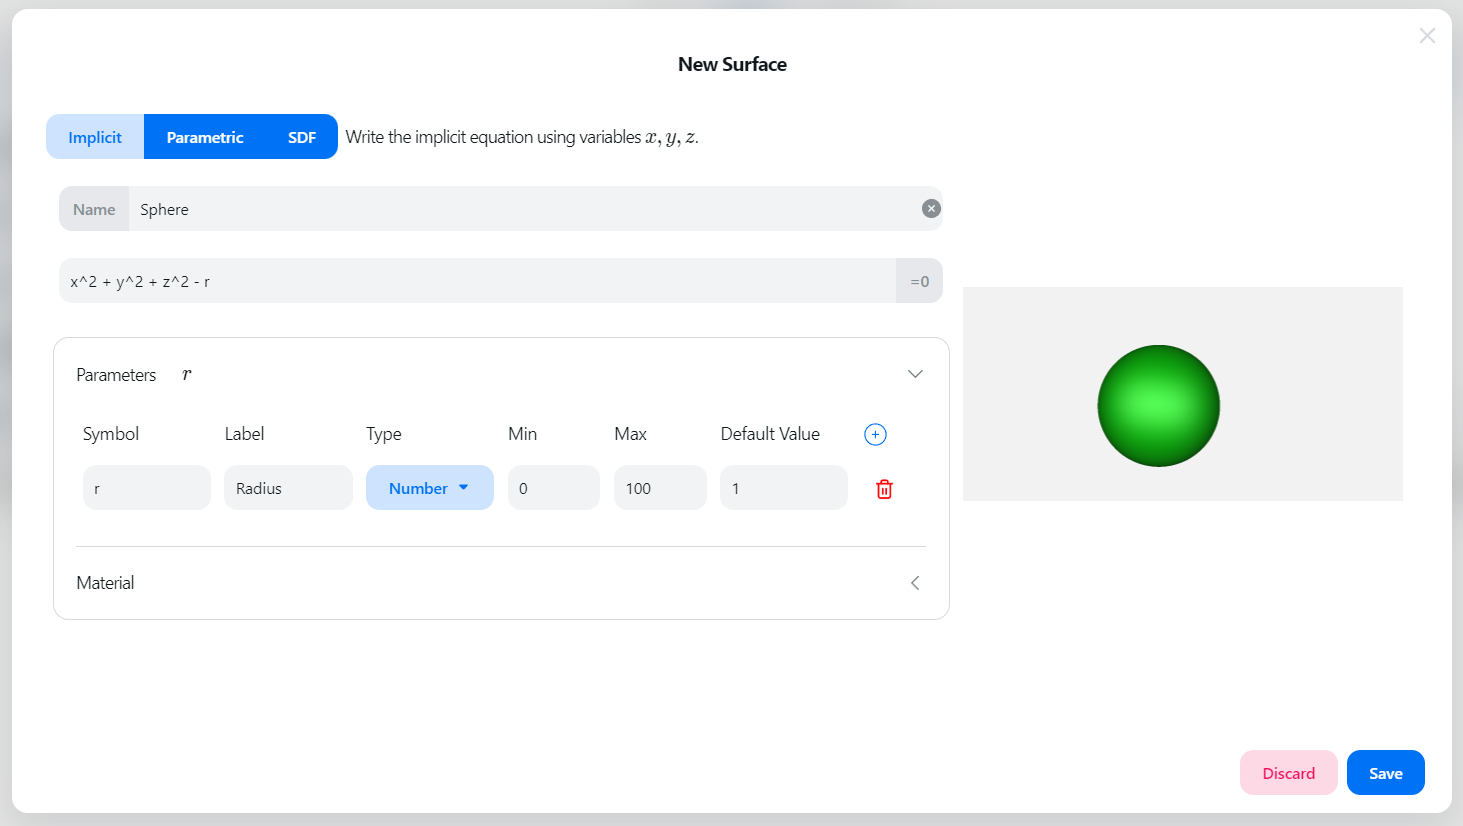
\includegraphics[width=\textwidth]{Plantilla-TFG-master/img/panel.png}
    \caption{Diálogo de edición de primitivas}
\end{figure}

El componente cuenta con una instancia del componente \texttt{Lienzo} para que el usuario pueda previsualizar la superficie que está definiendo. Como sabemos, el lienzo recibirá como argumento un manejador de excepción para actuar en caso de error de compilación. En caso de error, el manejador pasará el mensaje de error al componente y se lo indicará al usuario en el campo correspondiente.\newline
\begin{figure}[ht!]
    \centering
    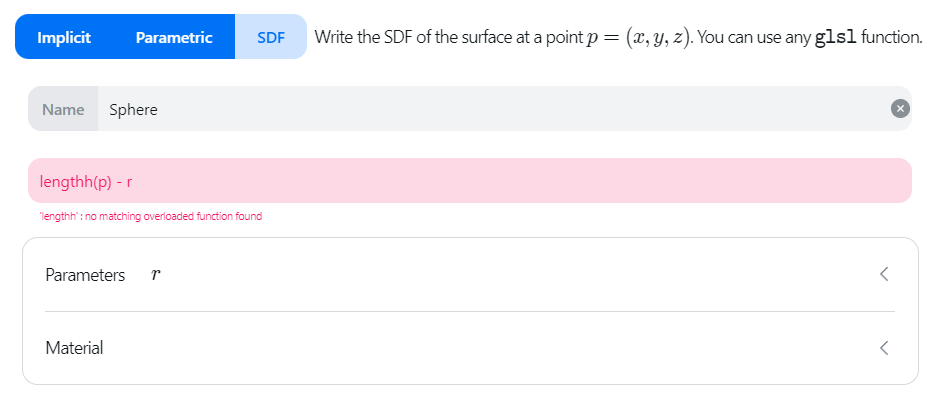
\includegraphics[width=\textwidth]{Plantilla-TFG-master/img/error.png}
    \caption{Ejemplo de error al usar un parámetro no definido}
\end{figure}

La forma de obtener la función distancia dependerá del método de entrada elegido por el usuario. La manera más directa es a través del modo \textbf{SDF}, en el que el usuario introduce la función distancia con signo con sintaxis GLSL y es pasada directamente al lienzo. La principal ventaja de este modo de entrada es que el el usuario puede hacer uso de todas las primitivas y operadores existentes, como muestra la \autoref{fig:repeat}\newline
\begin{figure}[ht!]
    \centering
    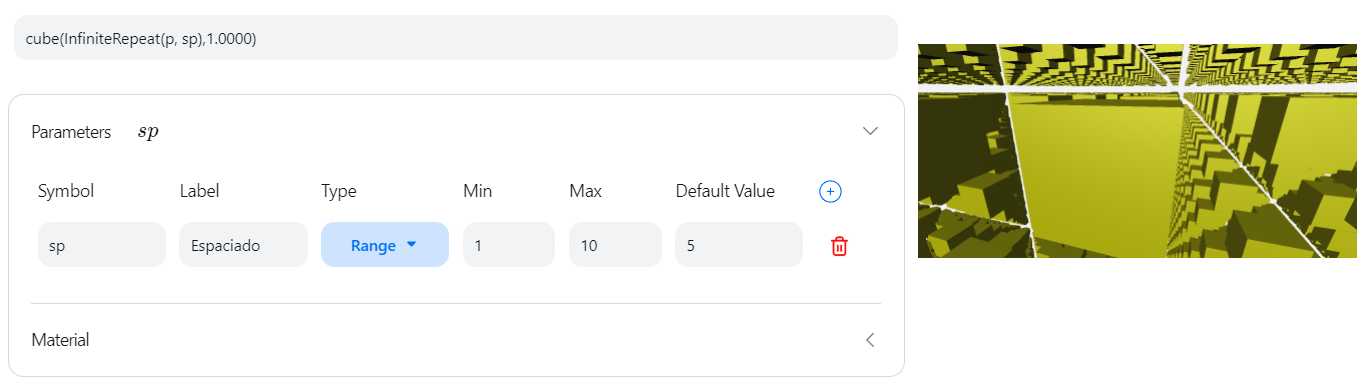
\includegraphics[width=\textwidth]{Plantilla-TFG-master/img/repeat.png}
    \caption{Ejemplo de creación en el modo SDF}
    \label{fig:repeat}
\end{figure}

La siguiente forma de definir una superficie es a través de su \textbf{ecuación implícita}, que el usuario deberá introducir en las variables $x,y,z$. En este caso, lo que recibirá el componente del lienzo será la cota función distancia con signo obtenida en la \autoref{p:aproxImp}. Para obtenerla volveremos a hacer uso de \texttt{nerdamer}, pues nos permitirá calcular el gradiente y su norma de forma más directa. La función que calcula esta cota es la siguiente.
\begin{lstlisting}[language=JavaScript, caption=Obtención de cota de ecuación implícita]
function ImplicitToSDF(implicit: string, parameters: Parameter[], evaluate: boolean = false) : string{
  let f: string | null = null; // Parsed string by nerdamer
  let res = "";

  try {
    f = nerdamer(implicit).toString();
  } catch (error: any) {
    error = error.message.split("at ")[0];
    throw new Error(`ERROR PARSING EQUATION ${implicit}`);
  }

  // Calculamos norma
  const dfdx = nerdamer.diff(f, "x", 1);
  const dfdy = nerdamer.diff(f, "y", 1);
  const dfdz = nerdamer.diff(f, "z", 1);
  const norm = nerdamer(`sqrt((${dfdx})^2 + (${dfdy})^2 + (${dfdz})^2)`);

  // Comprobamos que podemos dividir por la norma
  if (norm.toString() === "0") {
    throw new Error("NORM CAN'T BE 0");
  }
  else{
    let sdf = nerdamer(`(${f})/(${norm})`);
    var x = nerdamerTS.tree(sdf.toString());
    res = StringToSDF(x, parameters, evaluate);
  }

  return res;
}
\end{lstlisting}
El resultado que nos proporciona \texttt{nerdamer} no puede ser pasado directamente al lienzo, ya que no está en sintaxis GLSL. Tampoco podemos pasar la cadena de texto que nos proporciona su método \texttt{toString()}, ya que funciones como las potencias vendrían escritas como \texttt{a\textasciicircum b}, lo que en GLSL es el \texttt{OR} exclusivo bit a bit. El objetivo de la función \texttt{StringToSDF} es el de tener en cuenta estos casos especiales para así devolver una sentencia GLSL válida. Para ello recibe el árbol de la expresión de \texttt{nerdamer}, y de forma similar a como buscábamos monomios en el constructor de la clase \texttt{Polynomial}, ahora buscaremos los operadores que nos interese sustituir. Por ejemplo, en el caso de la potencia deberemos buscar el nodo con el operador \textasciicircum\ y escribir \texttt{pow(a,b)}, donde \texttt{a} y \texttt{b} son el resultado de expandir en preorden los hijos a izquierda y derecha respectivamente de dicho nodo. Por último, dado que en este componente el usuario no introduce valor para los parámetros, la función \texttt{StringToSDF} incluye la posibilidad de evaluar los parámetros en su valor por defecto para así poder pasar esta expresión al lienzo de previsualización. En el caso del editor de nodos esto no será necesario, pues el usuario indicará el valor de los parámetros.\newline

La última forma de definir una superficie es a través de su \textbf{parametrización racional}. En este caso el usuario tendrá varios campos de texto para introducir las ecuaciones de cada variable $x$, $y$, $z$, y podrá usar las variables $s,t$ en las ecuaciones. Usando el método \texttt{implicitateR3} de la clase \texttt{Ideal} 
obtenemos la ecuación implícita de la superficie, de la que podremos obtener una cota inferior con el procedimiento descrito anteriormente para pasarla como argumento al lienzo. En caso de que la parametrización no venga representada por una sola ecuación implícita, el método \texttt{implicitateR3} devolverá un error y su mensaje será mostrado al usuario.\newline

En la parte inferior del cuadro de diálogo se permite al usuario modificar los valores del material para la previsualización, así como crear y modificar los parámetros que desee. Para crear un parámetro se deberá indicar el símbolo que tiene este en la expresión de la función distancia, una etiqueta para mostrarlo en el editor de nodos, un valor por defecto y el método de entrada que tendrá el usuario para indicar  su valor en el editor de nodos. Si se elige la entrada por valor el usuario introducirá su valor en un campo de entrada numérica convencional. Si por el contrario se elige la entrada en un rango, en el editor de nodos aparecerá un deslizador, cuyos límites serán indicados por el usuario al momento de definir el parámetro.\newline

En todo momento se comprueba que el usuario esté introduciendo información válida, capturando posibles errores de \texttt{nerdamer} o de \texttt{multivariate-polynomial}. En caso de que se detecte algún error, se le indica al usuario en el campo correspondiente el mensaje. Un ejemplo de comprobación adicional a las que se realizan al calcular la función distancia es la siguiente. Dado que el identificador se calcula a partir del nombre que introduzca el usuario, no se podrá elegir ningún nombre cuyo identificador asociado ya esté asignado a otra primitiva diferente.\newline

Una vez toda la información introducida es válida, se le permite al usuario pulsar el botón de guardar. Esta acción hará que se llame a la función del contenedor de primitivas correspondiente, haciendo que se sobreescriba la primitiva original con la calculada para la previsualización (sin realizar la evaluación de los parámetros) y se reflejen los cambios tanto en el editor de nodos como en la tabla de primitivas. Finalmente, observar que en caso de que el usuario quiera crear una primitiva en lugar de editar una existente, el funcionamiento interno será el mismo, con la única excepción de que el cuadro de dialogo aparecerá completamente vacío.

